% M. S. Tsoeu (2011), University of Cape Town <mohohlo.tsoeu@uct.ac.za>

% This is a project report templace document created for EEE4022FS students at the University of Cape Town.
%
% This file should be is processed with ``pdflatex`` and might need a few modifications if a different processor is chosen.


\documentclass[a4paper,12pt]{report}


%Include packages you need to use here

\usepackage[top = 1in, bottom = 1in, left = 1in, right = 1in]{geometry}
\usepackage{graphicx}
\usepackage{fancyhdr}
\usepackage{amsmath, amsthm, amssymb}
\usepackage{lastpage}
\usepackage{subfigure}
\usepackage{lscape}
\usepackage{hyphenat}
\usepackage{setspace}
\usepackage{hyperref}
\usepackage{gensymb}
\usepackage{float}
\usepackage{ragged2e}
\usepackage[T1]{fontenc}
\usepackage[utf8]{inputenc}
\usepackage{lmodern}
\usepackage{minted}
\usepackage[T1]{fontenc}
\usepackage{titlesec, blindtext, color}
\usepackage{pdfpages}
\usepackage[tocflat]{tocstyle}
\usetocstyle{standard}
\usepackage{blindtext}
\usepackage{tocloft}

\usepackage{natbib}
\setlength{\bibsep}{1mm}

\begin{document}
% Include page formatting here. 
\parskip = 6mm
\parindent = 0mm
\renewcommand{\headrulewidth}{0pt}
\rhead[]{\thesection}
\lhead[\thechapter]{}


\definecolor{gray75}{gray}{0.75}
\newcommand{\hsp}{\hspace{20pt}}
\titleformat{\chapter}[hang]{\vspace{-20mm}\Huge\bfseries}{\thechapter\hsp\textcolor{gray75}{|}\hsp}{0pt}{\Huge\bfseries}

% This section formats the title page of the Report.
\thispagestyle{empty}
{\Huge \begin{center}
% Modify the line below to insert your title.
Servo Electronics Controller Board
% Modify the line below to insert your subtitle.
\end{center}}

\vskip 5mm
\begin{center}

\includegraphics[scale = 0.3]{uctLogo.png}
\end{center}

\vskip 5mm
\begin{center}
by Nicholas Antoniades		% Insert your name here
\end{center}

\vskip 5mm
\begin{center}
Prepared for Justin Pead\\ 		% Insert your supervisor's name here.
Dept. of Electrical and Electronics Engineering\\University of Cape Town
\end{center}


\vskip 10mm
\begin{center}
Submitted to the Department of Electrical Engineering at the University of Cape Town in partial fulfilment of the academic requirements for a Bachelor of Science degree in Mechatronics Engineering.

\end{center}

\vskip 5mm
\begin{center}{\bf \today}
\end{center}
\thispagestyle{empty}
\mbox{}
\newpage

\onehalfspacing
\thispagestyle{empty}
\vskip 40mm


% Please leave the declaration as it is (Standard UCT declaration).
{\Large Declaration}\\
\hrule

\vskip 10mm
\begin{enumerate}
\item I know that plagiarism is wrong. Plagiarism is to use another's work and pretend that it is one's
own.
\item I have used the IEEE convention for citation and referencing. Each contribution to, and quotation in,
this report from the work(s) of other people has been attributed, and has been cited and
referenced.
\item This report is my own work.
\item I have not allowed, and will not allow, anyone to copy my work with the intention of passing it off
as their own work or part thereof.
\end{enumerate}
\vskip 10mm
Signature:
\vspace{-21mm}
\begin{figure}[H]
  \hspace{23mm}  
\includegraphics[width=0.2\textwidth]{Signture.png}
\end{figure}
\vspace{-10mm}
\\N. Antoniades
\vskip5mm
Date: \today


\fancyfoot[C]{\thepage}
\pagestyle{plain}
\newpage
\pagenumbering{roman}


\vspace*{20mm}
{\Large Abstract}\\
\hrule
\begingroup
The purpose of this study is design a servomotor controller board that has all the functionality of the more expensive servomotor devices but costs much less.

The controller board allows for more advanced control of the servomotor, with serial communication hardware, and temperature and current sensors controlled by an on-board microcontroller. A master controls multiple slaves, communicating a change in position or a requested for information.The on-board power supply has a wide current range allowing for capability with a large range of servomotors.

All the components except the buck converter were successfully tested through building the circuit on the bread board. It was found that the pad spacing between the IC pins did not have solder mask. This led to the PCB being unsuccessful as the pins would short when power and ground were connected. This issue can be avoided by ensuring solder mask is applied between pads.

The designed system worked cost substantially less than more common servomotor controller boards. when tested all modules of the system worked but a second PCB design needs to be created in order to build a functioning prototype.
\endgroup
\vspace*{\fill}











\tableofcontents


\newpage
\listoffigures

\newpage
\listoftables

% Page formatting, to place section titles as headers of odd pages and Chapter titles as headers of even pages.


\pagenumbering{arabic}

% The files included below are .tex files containing the respective chapters these are already created in this package and you can add to or modify them.
\chapter{Introduction}

\vspace{10mm}
\section{Background to the study}
\vspace{5mm}
With advancements in technology, the demand for a robotic solution when problem solving is increasing fast and is already in high demand. Unfortunately the current hardware available in the market for accurate motor control is expensive, resulting in the only consumers who have access to it, being the large companies and other organisations with big budgets. This limits those individuals who want to design and prototype robotic applications at home or at university for research projects. 

These motor controller boards allow for more advanced control of the motor, not just direction control, they also allow for velocity, current and torque control with the aid of additional sensors. This helps give better performance and a higher accuracy of motor control. , allowing for more advanced robotic application.

There is a high demand for robotic software and hardware but until recent years it has been unaffordable for the general public. The aim of this study is to design and create an affordable servomotor controller board that will have all the functionality alike that of the more expensive controllers, but be much cheaper.   

\newpage
\section{Objectives of this study}
This project illustrates the design and production of a servomotor controller board. On-board sensors and microcontroller will be used to monitor temperature and current drawn as well as allow for motor control. The controller will be able designed to be cable of connecting to a wide range of servomotors as well as allowing multiple boards to be daisy chained together and be capable of serial communication. Advanced servomotor controllers are expensive. The designed board needs to have the abilities of the more expensive controllers, but be much cheaper. 

\vspace{5mm}
\section{Scope and Limitations}
The design of the controller board was performed from an academic view-point. The main goal being to create a proof of concept, showing that it is possible for cheaper servomotor controllers to be designed with the same functionality of more expensive controller boards.

\vspace{5mm}
\section{Plan of development}
This report is organised in the following order. First the objectives of the study and the problem to be solved are outlined in the Introduction. Second, a review of available literature on the topic at hand. The required system is then designed and components are chosen. The components are tested and the method and results are discussed. The PCB is the designed and the component placement and testing is discussed. The methods for the implementation of the code is discussed and then finally comclusion are drawn and recommendations were made. 




\chapter{Literature Review}

\vspace{-15mm}
\section{Servomotors}
\vspace{-5mm}
Typically servomotors are rotary or linear actuators that are controlled using a microcontroller and an encoder. This allows for the precise angular position, velocity and/or acceleration control of the output shaft. Servomotors are commonly used in motoring applications such as 3D printing and CNC machines, or in robotic arms and assemblies which use forward and reverse kinematics in order control specific motor positions allowing for complex tasks to be completed accurately\cite{servo}.
\vspace{-5mm}
\begin{figure}[H]
  \centering
  \begin{minipage}[b]{0.45\textwidth}
  \centering
    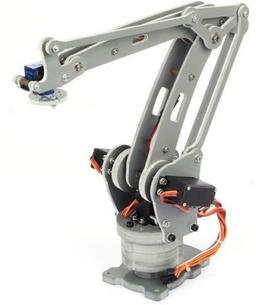
\includegraphics[width=0.35\textwidth]{servo_arm.jpg}
    \caption{Servo controlled arm  \cite{servo_arm}}
  \end{minipage}
  \hfill
  \begin{minipage}[b]{0.45\textwidth}
    \centering
    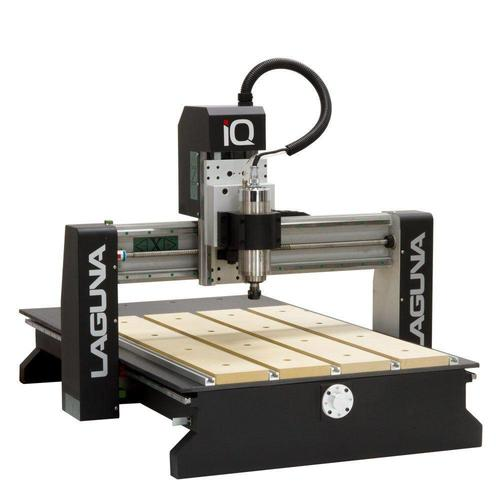
\includegraphics[width=0.5\textwidth]{cnc.jpg}
    \caption{CNC machine \cite{cnc}}
  \end{minipage}
\end{figure}
\vspace{-8mm}
A servomotors usually has 3 wires, Control, Power and Ground. The output shafts angle is controlled through adjusting the duty cycle of a Pulse Width Modulated (PWM) signal being supplied to its control wire. The on board microchip receives this signal and in turn outputs a voltage to a DC motor based on the duty cycle of the signal. This voltage rotates the motors shaft, which in turn rotates the output shaft to a specific angle, usually  between 0\degree and 180\degree but there are also servos that have it outputs a voltage 360\degree  of rotation. This position is tracked and controlled using an encoder such as a potentiometer in order to determine current position, but there are many other types of encoders which can give more accurate position, direction of rotation and velocity control. A typical servomotor and its components can be see in Figure \ref{fig:servoexplode} and Table \ref{tab:servomotorcomponents}. 
\vspace{-3mm}
\begin{figure}[H]
  \begin{minipage}[b]{0.48\textwidth}
    \begin{figure}[H]
        \centering
        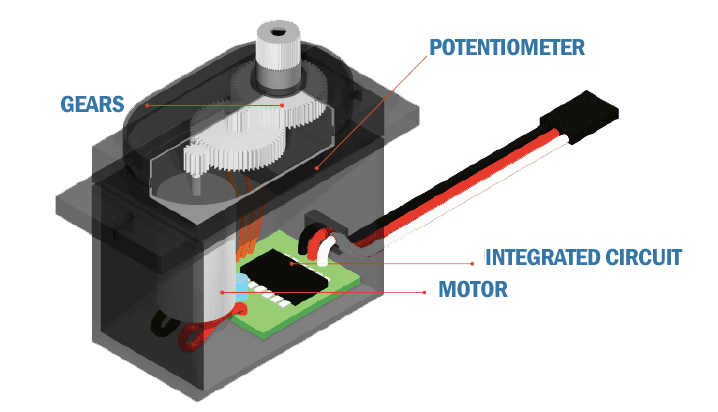
\includegraphics[width=0.8\textwidth]{Servoexploded.png}
        \caption{Servomotor components\cite{servoexplode}}
        \label{fig:servoexplode}
    \end{figure} 
\end{minipage}
\hfill
\begin{minipage}[b]{0.48\textwidth}
  \
    \begin{table}[H]
        \centering
        \begin{tabular}{|l|}
        \hline
        \textbf{\underline{A servomotors components}}\\
             - A Motor(AC/DC) \\
             - Potentiometer as the encoder \\
             - A microcontroller for control \\
             - A Gear train \\
         \hline
        \end{tabular}
    \caption{Servomotor components }
    \label{tab:servomotorcomponents}
    \end{table}
  \end{minipage}
\end{figure}
\vspace{-10mm}

\newpage
\section{DC motors}
A current carrying conductor within a magnetic field will experience a force. The direction of the force will be perpendicular to the plane containing the current carrying conductor and it's magnetic field which are also perpendicular to each other. This is the principle used in a simple brushed DC motor with permanent magnets used for poles and a slip ring commutator to alternate the flow of the current on the conductor. Power to the coils is supplied through fixed conductive brushes that make contact with the rotating commutator. The force rotates the shaft at a rate related to the voltage applied to the motor\cite{DC_Motor}.
\begin{figure}[H]
\centering
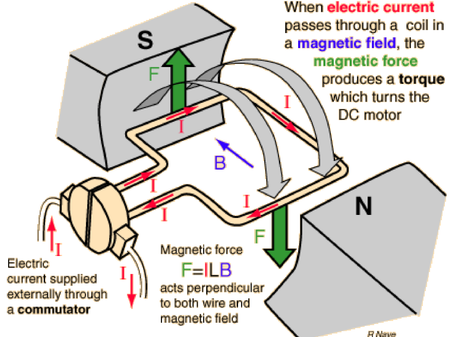
\includegraphics[width=0.5\textwidth]{lorenzforce.png}
\caption{Current carrying conductor in a magnetic field\cite{DCmotor}}
\end{figure} 
With brushless DC motors the rotor is a permanent magnet, the rotor is then rotated by rotating the surrounding magnetic field. Brushless motors have a higher power to weight ratio and high speed control. They do not miss steps and are much more powerful and efficient, but cost a lot more than brushed DC motors  \cite{brushlessDC}
\begin{figure}[H]
\centering
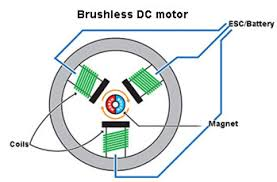
\includegraphics[width=0.45\textwidth]{Brushless_DC.jpeg}
\caption{Brushless DC motor \cite{brushlessDC}}
\end{figure} 


\newpage
\section{Microcontrollers}
A microcontroller acts as the brain of the system, using different peripherals to interact with different devices and being able to make decisions in order to perform tasks. The hardware integrated with microcontroller and the quality of the software loaded determines how well it functions and tasks it can perform.

\subsection{Flash Memory}
Flash memory is an electronic non-volatile computer storage medium that can be electronically erased and reprogrammed. Flash memory contains its information even when the device is not powered. What is included in this is information required to start up the micro and be active during runtime.

The Flash memory on the STM32F051C6 has been organised into 32-bit wide memory cells that can be used for storing both code and data constants.

\textbf{This information is divided into two parts :}
\begin{enumerate}
\item{\textbf{System memory}}
which is used to boot the device on start-up in System memory boot mode. This area is reserved for use by the manufacturers of the microcontroller, and contains the boot loader which is used to reprogram the Flash memory through the selected communication interface. It is programmed by ST when the device is manufactured, and protected against various write/erase operations. 

\item{\textbf{Optional bytes}}
that include those used when re-programming the device for specific applications.
\end{enumerate}

\subsection{DAC}
Digital-to-analog converters are used to create an analog signal based on a digital value. The most basic type of electronic DAC uses pulse-width modulation and a low pass filter. A chosen stable current or voltage is achieved by adjusting the frequency of the PWM signal. The duty cycle of the PWM based on the value of digital input. This technique is often used for electric motor speed controllers and other applications \cite{DAC}.

\newpage
\subsection{ADC}
An analogue-to-digital converter(ADC) allows for a voltage source to be sampled and read in to the microcontroller as digital code. The resolution of the ADC determines the number of bits used to specify a certain voltage range e.g. for an ADC with $2^8$ bit having a resolution 255. If the voltage range to be sample is between 0V and 3.3V. Gives a resolution of 12.9mV per bit.

\subsubsection{Successive Approximation Converters}
Successive approximation ADCs are a type of analog-to-digital converter that reads in a continuous analog signal and outputs a digital binary value based on the input signal. This type of converter uses a binary search through all the possible quantization levels. The SAR outputs a binary value of the approximated ADC value, which is then converted back into an analog signal and compared to the input wave form using a comparator. If the signals are not the same the SAR increments its approximation until converging upon the final digital value to be output. Once this occurs an End Of Conversion (EOC) signal is sent to the microcontroller.

The STM32F051C6 uses a Successive Approximation ADC like the one seen below in Figure \ref{fig:SAC}.
\begin{figure}[H]
    \centering
    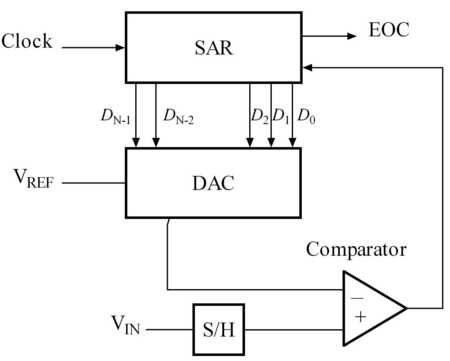
\includegraphics[width=0.5\textwidth]{SA_ADC_block_diagram.jpg}
    \caption{Successive Approximation Converters \cite{SA_converter}}
    \label{fig:SAC}
\end{figure}





\newpage
\section{Sensors}
Multiple sensors will be incorporated into the final design of the controller board. Sensors are important in the functioning and accurate control of the system as well as allowing for protection against overheating and excess current draws. 

\vspace{-7mm}
\subsection{Current sensor}
A current sensor is a device that detects electric current and generates a signal in proportion to that of the current, the output of the sensor can be analogue or digital \cite{current_sensor}. 

\textbf{Typical current sensors that are available:}  
\begin{table}[H]
    \centering
    \begin{tabular}{|c|c|}
    \hline
    &\\
      \begin{minipage}[b]{0.45\textwidth}
            \begin{figure}[H]
                \centering
                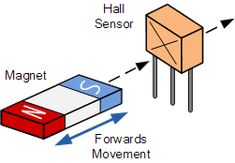
\includegraphics[width=0.5\textwidth]{Hall_Effect.jpg}
                \caption{Hall sensor}
                \label{fig:hall}
            \end{figure}

      \end{minipage}
         & 
      \begin{minipage}[b]{0.45\textwidth}
           \textbf{Hall effect sensors}, seen in Figure 2.7. can be used to measure the magnetic field made created by the current flowing through conductor and from that determine the actual current. \newline
      \end{minipage}\\

      \hline      
      \begin{minipage}[b]{0.45\textwidth}
          \textbf{Shunt resistors}, seen in Figure 2.8. Use Ohms law in order to calculate the current flowing. $V = I\times R$, with a known applied voltage and chosen resistor the current can be calculated.\newline
      \end{minipage}
         &  
        \begin{minipage}[b]{0.45\textwidth}
            \begin{figure}[H]
              \centering               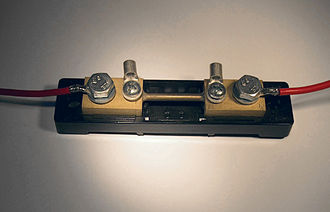
\includegraphics[width=0.6\textwidth]{shunt_resistor.jpg}
                \caption{Shunt resistor}
                \label{fig:shunt}
            \end{figure}
        \end{minipage}\\
        \hline        

          \begin{minipage}[b]{0.45\textwidth}
          \begin{figure}[H]
            \centering
            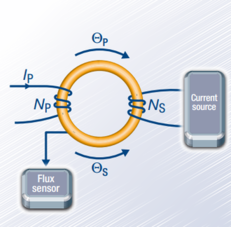
\includegraphics[width=0.5\textwidth]{saturable_inductor.png}
            \caption{Saturable inductor}
            \label{fig:Saturable}
          \end{figure}
          \end{minipage}
         &  
           \begin{minipage}[b]{0.45\textwidth}
            \textbf{Saturable inductor sensors}, seen in Figure 2.9. Work in a similar manner to that of Hall effect sensors in that they measure the change in the magnetic field in order to determine the current flowing through a conductor.
            \vspace{6mm}
          \end{minipage}
         \\
     \hline
    \end{tabular}
    \vspace{2mm}
    \caption{Types of current sensor}
\end{table}


\newpage
\subsection{Encoders}
Encoders are electromechanical devices that output an electrical signal proportional to that of the position of the input shaft.

\textbf{Typical encoders that are available:}  
\vspace{5mm}
\begin{table}[H]
    \vspace{-5mm}
    \centering
    \begin{tabular}{|c|c|}
    \hline
      \begin{minipage}[b]{0.49\textwidth}
      \vspace{2mm}
        \textbf{Optical encoders}, which use pulses of light emitted by infrared diodes shining through slots. This can be seen in Figure 2.10 As the number of slots increases so does the encoders resolution\cite{encoders}.
        \vspace{5mm}
      \end{minipage}
         & 
      \begin{minipage}[b]{0.49\textwidth}
      \begin{figure}[H]
        \centering
        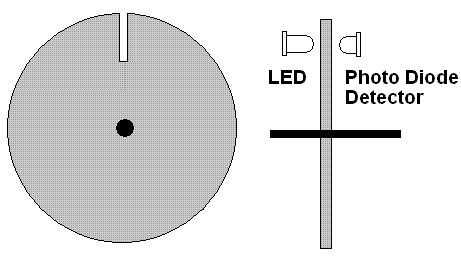
\includegraphics[width=0.6\textwidth]{slottedencoder.png}
        \caption{Optical encoder}
        \label{fig:optical}
      \end{figure}
      \end{minipage}\\
      \hline   
      
      \begin{minipage}[b]{0.45\textwidth}
      \centering
      \begin{figure}[H]
          \centering
            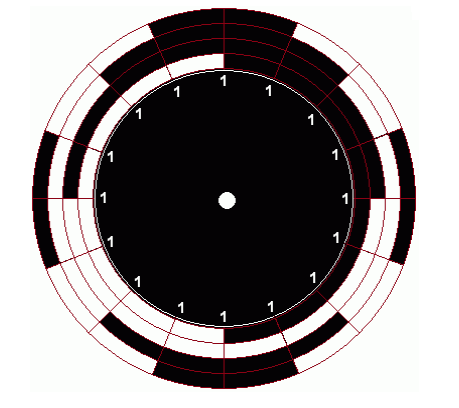
\includegraphics[width=0.49\textwidth]{Graycodeencoder.png}
            \caption{Binary encoder}
            \label{fig:binenc}
      \end{figure}

      \end{minipage}
         &  
        \begin{minipage}[b]{0.49\textwidth}
        \vspace{2mm}
              \textbf{Binary encoders}, which uses a template that has segments based on a binary value to determine current position. This can be seen in Figure 2.11. multiple motor positions can be determined, the number of positions has a $2^N$ relationship with the number of segments in the encoder. 
              \vspace{2mm}
        \end{minipage}\\
         \hline
          \begin{minipage}[b]{0.49\textwidth}         
            \textbf{Potentiometers}, are a mechanical encoder. This can be seen in Figure 2.12. Where the different resistance values and there associated voltage represent different position values of the wiper on the resistive strip \cite{rotarypot}.
        \end{minipage}
         &
          \begin{minipage}[b]{0.49\textwidth}
          \centering
              \begin{figure}[H]
              \centering
                 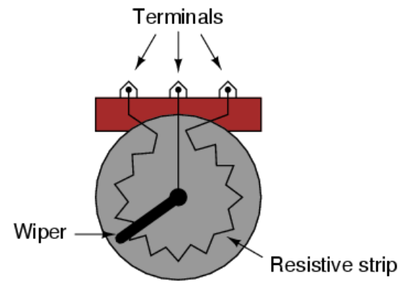
\includegraphics[width=0.5\textwidth]{Rotarypot.png}
                    \caption{Potentiometer}
                    \label{fig:pot}
              \end{figure}

 
        \end{minipage}
         \\
         \hline
          \begin{minipage}[b]{0.49\textwidth}
          \centering
          \begin{figure}[H]
          \centering
             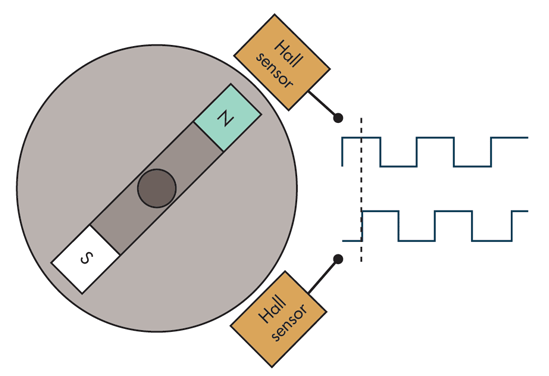
\includegraphics[width=0.4\textwidth]{Halleffect.png}
             \caption{Hall effect encoder}
             \label{fig:hallenc}
          \end{figure}
         \end{minipage}
         &
          \begin{minipage}[b]{0.49\textwidth}
          \vspace{5mm}
          \textbf{Hall effect sensors}, are transducers that have an output voltage that varies in response to a magnetic field. Seen in Figure
          2.13. This us then used to determine position and velocity\cite{halleffect}. 
          \vspace{5mm}
          \end{minipage}
         \\
         
     \hline
    \end{tabular}
    \vspace{-4mm}
    \caption{Types of encoders}
\end{table}
\vspace{-10mm}



\newpage
\subsection{Temperature sensors}
Temperature sensors are an important way to monitor and keep track of the state of the device during different operating conditions.

\begin{itemize}
	\item[-]Analogue temperature sensors output a voltage that depends on the temperature of the device and this can be read using the ADC of a microcontroller and then the devices temperature can be calculated. 
    \item[-]Digital temperature sensors will communicate the temperature at the sensor using I2C or another form of communication.
\end{itemize}

\textbf{Typical temperature sensors that are available:}  

\begin{table}[H]
    \centering
    \begin{tabular}{|c|c|}
    \hline
    &\\
      \begin{minipage}[b]{0.45\textwidth}
          \textbf{Thermocouples}, use two different wires made of different metals connected at two points. The varying voltage between two points, reflecting proportional changes in temperature \cite{Temprature_sensor}.
          \vspace{10mm}
      \end{minipage}
         & 
      \begin{minipage}[b]{0.45\textwidth}
      \begin{figure}[H]
           \centering
            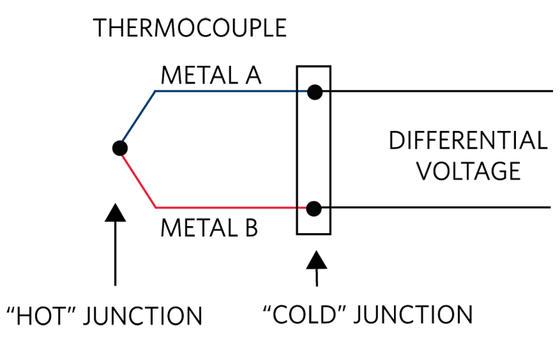
\includegraphics[width=0.8\textwidth]{Thermocouple.jpg}
            \caption{Thermocouple setup}
      \end{figure}

      \end{minipage}\\

      \hline      
      \begin{minipage}[b]{0.6\textwidth}
        \begin{figure}[H]
              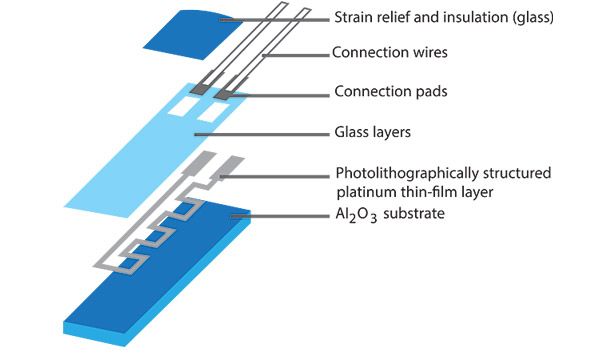
\includegraphics[width=1\textwidth]{RTD.jpg}
              \vspace{-5mm}
              \caption{RTD}
              \vspace{2mm}
        \end{figure}
      \end{minipage}
         &  
        \begin{minipage}[b]{0.39\textwidth}
            \textbf{Resistance Temperature Detectors (RTDs)}, measure temperature changes by correlating the resistance of the device element and temperature. An RTD consists of a film for greater accuracy, a wire wrapped ceramic or a glass core \cite{Temprature_sensor}. 
            \vspace{13mm}
        \end{minipage}\\
        \hline
    \end{tabular}
    \caption{Types of temperature sensors}
\end{table}

\newpage
\section{Communication}
Traditionally when connecting multiple servomotors to a microcontroller, each servo must be individually connected to the micro, and each servo must individually be connected to the power supply. This can result in long masses of wires when multiple servomotors are used in one project, seen in Figure 2.16. This also limits the number of servomotors that can be controlled at a time to the number of GPIO pins available on the microcontroller.

\begin{figure}[H]
\centering
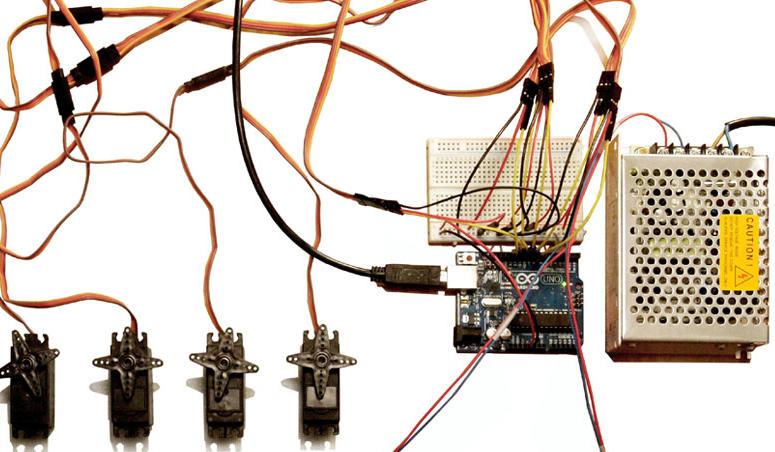
\includegraphics[width=0.4\textwidth]{toomanywires.jpg}
\caption{Multiple servomotors connected to one microcontroller\cite{toomanywires}}
\label{fig:typset}
\end{figure}

The controller board that will be designed to enable that the servo motors to be connected in series and be able to communicate using the RS485 differential serial communication standard. This will allow for communication over a longer distances with a high noise rejection for increased accuracy. This enables the master to effectively communicate to each individual slave a certain position value and request information such as current drawn or temperature at the motor from it in return. The Master and Slave servo inter-connection can be seen below in Figure \ref{fig:servoconnection} \newline

\begin{figure}[H]
\centering
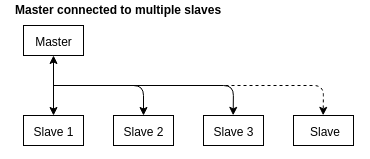
\includegraphics[width=0.6\textwidth]{master_slave.png}
\caption{Servo inter-connection}
\label{fig:servoconnection}
\end{figure}

The RS485 standard is a hardware protocol that will require that the microcontroller interacts with a transceiver which will be able to facilitate the communication. 


\newpage
\subsection{Serial communication}
Serial communication is the process of sending data one bit at a time, from one device to another sequentially over a communication channel or a computer bus \cite{serial_comms}. Communication is accomplished using 3 lines. (1) Ground (2) Transmit and (3)Receive. 

Serial communication can be synchronous or asynchronous. What this means is that the communicating devices either run off their own clocks and before hand decide on a common speed at which to communicate, this is asynchronous communication.  Or they will run off a common clock which will in turn give them a common communication speed,  this is synchronous communication. Asynchronous communication allows for information to be transmitted and received simultaneously. This is know as Full Duplex communication. Where as synchronous communication is Half Duplex communication and only one device can transmit information at a time. Serial communication can be used over much greater distances in comparison to other forms of communication, such as parallel communication, making it ideal in applications when communicating between devices that are far apart . 

\textbf{Serial communication is made of four parts :}
\begin{enumerate}
\item{\textbf{Baud rate}}
is the speed at which the communication occurs and it indicates the bits the number of bits transferred per second. Baud rate can also be read as the frequency of the clock needed for sampling, for example 3000 baud would mean the clock is running at 3kHz.
\item{\textbf{Data bits}}
are bits of information that needs to be transmitted.
\item{\textbf{Stop bits}}
are used to indicate the end of the communication for a single packet.
\item{\textbf{Parity}}
is used for error checking when using serial communication. There are four types of parity. Even, odd, marked, and spaced. When using even or odd parity the last bit after the data will be set to 0 or 1. Depending if it is even or odd parity. Then when a message is received its parity can be checked to check its accuracy. This can be used to detect noise and whether the communicating devices clocks are out of sync.

\end{enumerate}
\begin{figure}[H]
\centering
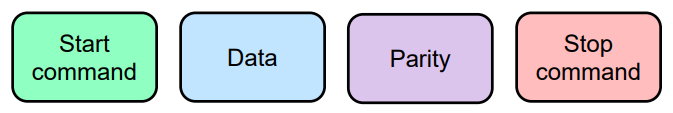
\includegraphics[width=0.6\textwidth]{serial.png}
\caption{Basic structure of a serial message}
\end{figure}

\newpage
\subsection{Recommended Standards}
When communicating using serial communication a Recommended Standard (RS) is typically used for easy connection between different devices. These standards use the Universal Asynchronous Receiver Transmitter (UART) hardware interface to facilitate the communication. Usually a UART is part of an integrated circuit (IC) and the signal level shifting needs to be handled by a driver circuit external of the UART. When communicating using a RS, a hardware interface is required in order to do the voltage level shifting. These components are known as level shifting transceivers. 

A simplified diagram of the implementation of asynchronous serial communication between two devices can be seen below in Figure 2.19.
\begin{figure}[H]
\centering
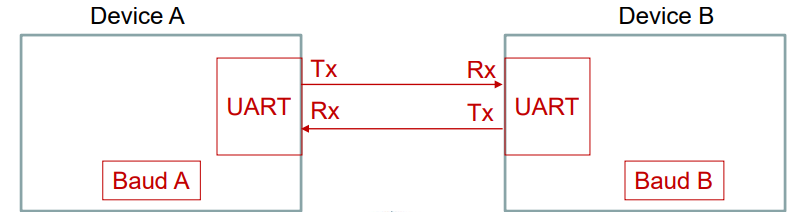
\includegraphics[width=0.8\textwidth]{UART.png}
\caption{UART communication between two devices }
\label{fig:comms}
\end{figure}

\textbf{Common Standards :}
\begin{enumerate}
\item{\textbf{RS232}}
Designed to work over a distance of up to 15 meters. The maximum baud rate is 19.2k. A logic level of -3v and less represents a 1 and 3v and more represents 0 \cite{RS232}.

\item{\textbf{RS422}}
Introduced to enable higher data rates than what was possible with RS-232 using differential transmitters and receivers. Works over a distance of up to 15m \cite{RS422}. 

\item{\textbf{RS485}}
RS-485 uses differential serial communication. Differential communication transmits information using two complementary signals over a twisted pair of conductors. Any external electromagnetic interference will then effect both conductors in the same way. Since the receiving circuit detects only the difference between the pair of conductors, the signal can be communicated more clearly and over greater distances \cite{Differential communication}. allowing for there to be up to 32 devices connected to a single serial communication line \cite{RS485}. 
\end{enumerate}

\newpage
\section{Buck Converter}
\vspace{-5mm}
According to Joule’s first law. The electrical current passing through a conductor  will generate heat with power that is proportional to resistance of the conducter and square of the current, $P=I^2\times R$. Therefore, in order to minimise power loss, the current drawn is reduced. In order to still transmit the same amount of power with the lower current, the voltage is increased as $P=V\times I$ \cite{High_voltage}. 

That is, in order keep power the same, while transmitting lower current, the voltage must be increased. Thus in order to be able to efficiently supply power to multiple servomotor controller boards, all the boards will be connected to a supply voltage in the range of 5V to 40V. Each board will have its own on-board buck converter to step down the voltage and step up the current in order to drive the servomotor and other components.

The power supply required for the designed board must be able to power the servo motor as well as the other on board components. This means that the supply must be able to handle the total current requirement of the board while still supplying the 5V required by the servo motor. Any other voltage requirements in the circuit will require a voltage regulator for further regulation.  

When considering the buck converter, the power demands of the servomotor was the greatest. The current drawn by the rest of the components was almost negligible in comparison. Table 2.5 was used to create an idea of a typical servomotors power consumption characteristics. This was used to help determine the current requirements of the designed buck converter.
\vspace{2mm}
\begin{table}[H]
        \centering
        \begin{tabular}{|c|c|c|c|}
        \hline
         \textbf{\underline{Name}}  & \textbf{\underline{Weight(g)}}   & \textbf{\underline{Stall Torque($\frac{kg}{cm}$)}} & \textbf{\underline{Stall Current(A})}\\
          MG90S   & 13.4 & 1.8  & 0.2  \\
          MG90    & 14   & 2    & 0.48 \\
          SG-5010 & 39   & 5.5  & 0.6  \\
          MG996R  & 55   & 9.4  & 2.5  \\
          MG946R  & 55   & 10.5 & 1.2  \\
          MG958   & 65   & 18   & 1.6  \\
          \hline
        \end{tabular}
        \caption{Current requirements of various servomotors}
\end{table}
\vspace{-5mm}
It was determined that the buck converter needed to be able supply 5V while outputting up to 4A worth of current in order to be able to run a range of different servo motors at stall torque as well as sufficiently power the rest of the circuit.

\subsection{Design Procedure}
Buck converters are a type of switch mode power supply that step down a higher voltage to a lower voltage. This is achieved through high frequency switching of the circuit with the source voltage with the help of a few added necessary components. 

The kind of switching required by the buck converter is typically achieved with a high speed MOSFET. A microcontroller supplies a PWM signal of the right frequency to the gate of the MOSFET, the duty cycle of the PWM signal determining the length of time of which the switch will stay open and closed. A basic buck converter circuit can be seen in Figure \ref{typbuck}.
\begin{figure}[H]
    \centering
    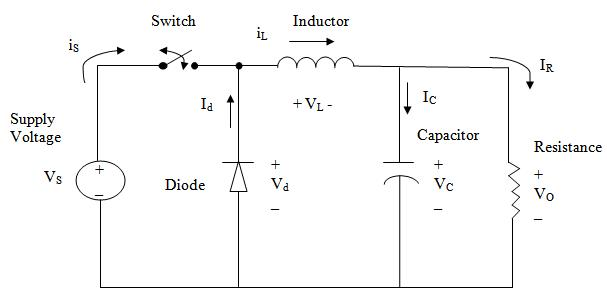
\includegraphics[width=0.85\textwidth]{buckconverter.JPG}
    \caption{A basic buck converter circuit \cite{buckconverter}}
    \label{typbuck}
\end{figure}
\vspace{-2mm}
In order to sufficiently meet design requirements, the design procedure requires that the following parameters need to be known or calculated :
\vspace{2mm}
\begin{table}[H]
        \centering
        \begin{tabular}{l l}
         \textbf{Parameters chosen}  & \textbf{Parameters needing to be calculated}\\
         $V_{IN(max)}$ = maximum input voltage & D =duty cycle\\
         $V_{OUT}$ = desired output voltage & \triangle _L = Inductor Ripple Current\\
         $I_{LIM(min)}$ = minimum current to the switch & $I_{MAXOUT} $ = Maximum IC output current \\
         $f_s$ = minimum switching frequency of IC &L = calculated inductor value \\
         $\mu = $ efficiency of the converter&$I_{SW(max)}$ = Maximum switch current\\
        \end{tabular}
        \vspace{2mm}
        \caption{Buck converter parameters}
\end{table}
\newpage
\subsection{Calculations}
\vspace{-2mm}
Once the desired buck converter IC, and input output parameters have been chosen. The following calculations can be done in order to solve for the components required to build the buck converter circuit. The calculations used for the design process of the buck are based on those found in the application  report  "Basic Calculation of a Buck Converter's Power Stage", made by Texas Instruments \cite{buck_calculations}.

\subsubsection{Maximum Switch Current}
\vspace{-6mm}
The first step to calculating the switch current is to determine the duty cycle, D, for the maximum input voltage:
\vspace{-5mm}
\begin{figure}[H]
    \centering
    $\mathbf{D = \frac{V_{OUT}}{V_{IN(max)}\times \mu}}$
\end{figure}
\vspace{-5mm}
The inductor ripple current is determined by chosen an inductor specified in the buck converters data sheet:
\vspace{-5mm}
\begin{figure}[H]
    \centering
    $\mathbf{\triangle I_L = \frac{(V_{IN(max)-V_{OUT}\times D})}{f_s\times L}}$ 
\end{figure}
\vspace{-5mm}
It needs to be determined if the chosen buck converter IC can deliver the required maximum output current:
\vspace{-5mm}
\begin{figure}[H]
    \centering
    $\mathbf{I_{MAXOUT} = I_{LIM(min)} - \frac{\triangle  I_L}{2}}$
\end{figure}
\vspace{-6mm}
If the maximum output current is above the maximum output current required for the device, the maximum switch current of the system must be calculated in order to determine the peak current that the inductor, switch and external diode must be able to withstand: 
\vspace{-5mm}
\begin{figure}[H]
    \centering
    $\mathbf{I_{SW(max)} = \frac{\triangle I_L}{2} + I_{OUT(MAX)}}$ 
\end{figure}
\vspace{-5mm}

\subsubsection{Inductor Selection}
\vspace{-6mm}
The buck converters data sheet will have a range of recommended inductor values, the higher the maximum output inductor, the higher the maximum output current due to reduced ripple. If no recommended inductor is given in the buck converters data sheet the following equation can be used:
\begin{figure}[H]
    \centering
    $\mathbf{L = \frac{V_{OUT} \times(V_{IN} - V_{OUT})}{ \triangle I_L \times{f_s} \times{ V_{in}}}}$
\end{figure}


\newpage
\subsubsection{Rectifier Diode}
\vspace{-2mm}
The chosen rectifier diode needs to be able to handle the fast switching and the current loads experienced during operation. The foreword current rating of the rectifier can be calculated using:
\vspace{-2mm}
\begin{figure}[H]
    \centering
    $\mathbf{I_F = I_{OUT(MAX)}\times(1-D)}$ 
\end{figure}
\vspace{-6mm}
Schottky diodes can be used to reduce the losses experienced, due to there fast switching capabilities and the low voltage drop across the diode.
The power that the chosen diode needs to be able to safely dissipate is calculated:
\begin{figure}[H]
    \centering
    $\mathbf{P_D = I_F\times V_F}$ 
\end{figure}
\vspace{-5mm}
\subsubsection{Output Voltage}
\vspace{-2mm}
Most buck converters set the output voltage with a resistive feedback divider network with resistors $R_1$ and $R_2$. This determines the feedback voltage $V_{FB}$. With $V_{OUT}$ the desired output voltage and the feedback bias current, $I_{FB}$, the resistors for the voltage divider can be calculated:
\begin{figure}[H]
  \begin{minipage}[b]{0.48\textwidth}
      \begin{figure}[H]
    \centering
    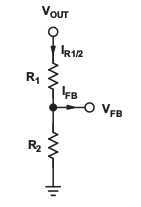
\includegraphics[width=0.35\textwidth]{Voltage_set.jpg}
    \caption{Resistive Divider}
    \end{figure}
  \end{minipage}
  \hfill
  \begin{minipage}[b]{0.48\textwidth}
    \begin{figure}[H]
    \hspace{10mm}
    $\mathbf{R = \frac{V_{FB}}{I_{R\frac{1}{2}}}}$ 
    \end{figure}
    \begin{figure}[H]
    \hspace{10mm}
    $\mathbf{R_1 = R_2 \times{( \frac{V_{OUT}}{V_{FB}} - 1)}}$ 
    \end{figure}
    \vspace{16mm}
  \end{minipage}
\end{figure}

\subsubsection{Input Capacitor}
\vspace{-2mm}
The minimum value of the input capacitor is normally given in buck converter ICs the data sheet. This is the minimum value necessary to stabilise the input voltage due to the peak current requirement of a switching power supply.

\newpage
\subsubsection{Output capacitor}
\vspace{-5mm}
The recommended value for the output capacitor is usually given in the buck converter ICs data sheet. The output capacitors value for a desired output voltage ripple is given by:
\vspace{-5mm}
\begin{figure}[H]
    \centering
    \large
    $\mathbf{C_{OUT(min)} = \frac{\triangle I_L}{\times f_s \times \triangle I_L}}$
\end{figure}
\vspace{-7mm}
If the output capacitors selection is based in transient response and not steady state ripple, the following formula can be used to calculate the output capacitance required for a desired minimum overshoot: 
\begin{figure}[H]
    \centering
    \large
    $\mathbf{C_{OUT(min),OS} = \frac{\triangle I_{OUT} \times L}{2 \times f_s V_{OUT} \times V_{OS}}}$
\end{figure}

\vspace{-9mm}
\section{Voltage Regulator IC}
\vspace{-5mm}
The on board components will run at the same or lower voltage than that of the servomotor and in order to step down the voltage an on board voltage regulator IC will be required.

Linear voltage regulators make use of a BJT or MOSFET device controlled by a high gain differential amplifier. The output voltage is compared to a reference voltage created by resistors R1 and R2 in Figure \ref{RESDIV} The output voltage is constantly adjusted to match this reference voltage in order to maintain a regulated output.  

Although the implementation of a linear regulator is simple, it is often a more inefficient method of regulation. The transistor or MOSFET acts as a resistor and any excess electrical energy is dissipated as heat\cite{linear_regulator}
\vspace{-4mm}.
\begin{figure}[H]
    \centering
    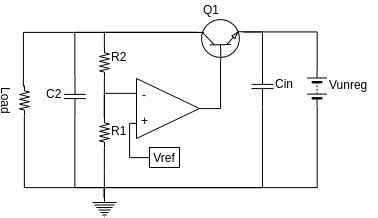
\includegraphics[width=0.55\textwidth]{Linear_Voltage_Regulator.jpg}
    \caption{Typical voltage regulator IC}
    \label{RESDIV}
\end{figure}
\vspace{-8mm}
It is common to find fixed three terminal linear regulators that generate a fixed standard voltage needed by common microcontrollers and peripherals such as the 3.3V or 5V without requiring any external components.

\newpage
\section{Related projects}
\subsection{Dynamixel}
The Dynamixel is an energy efficient high performance actuator that includes a controller, motor driver and network capabilities allowing multiple motors to be communicated to on a single channel.
\begin{figure}[H]
\centering
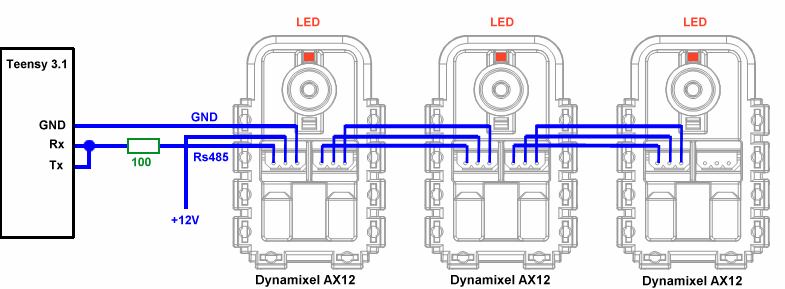
\includegraphics[width=0.7\textwidth]{Dynamixel.png}
\caption{Dynamixel connectors \cite{Dynamixel}}
\end{figure}

The Dynamixel allows for position and velocity control, as well as current based torque control of a brushless DC motor.  This allows for 360\degree  rotation with six standard operating modes ,although it can be programmed specifically for each application, this allowing for wide range implementation. Temperature and current tracking allow for shutdown protection. Due to high cost only larger companies and well funded organisations tend to have access to these devices. A standard Dynamixel actuator can cost up to R4500.\newline
 
\begin{figure}[H]
\centering
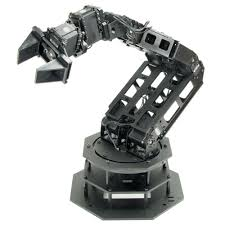
\includegraphics[width=0.35\textwidth]{Dynamixel_app.jpg}
\caption{Dynamixel based robotic arm  \cite{Dynamixel}}
\end{figure}


\newpage
\subsection{Odrive}
Odrive is a high performance servomotor controller board which uses a high resolution encoder with brushless DC motors in order to achieve  high accuracy position and velocity control. \newline

\begin{figure}[H]
\centering
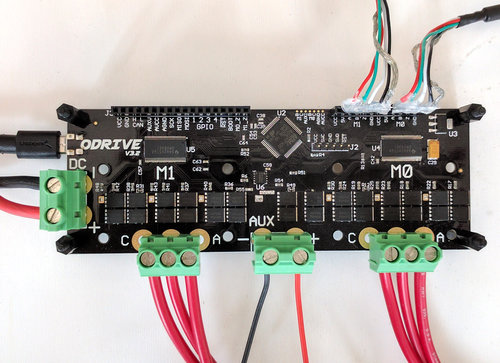
\includegraphics[width=0.5\textwidth]{odrive_board.jpg}
\caption{Odrive controller board\cite{Odrive}}
\end{figure}

The servomotor controller board can drive to motors. It allows for current, position and velocity control. Motor breaking can be achieved with a brake resistor and the board supports regenerative breaking. Communication with the board can be achieved with multiple interfaces, such as USB, UART, PWM and CAN. Although the Odrive is cheaper than the Dynamixel, it still costs R1800 for just the controller board.

\begin{figure}[H]
\centering
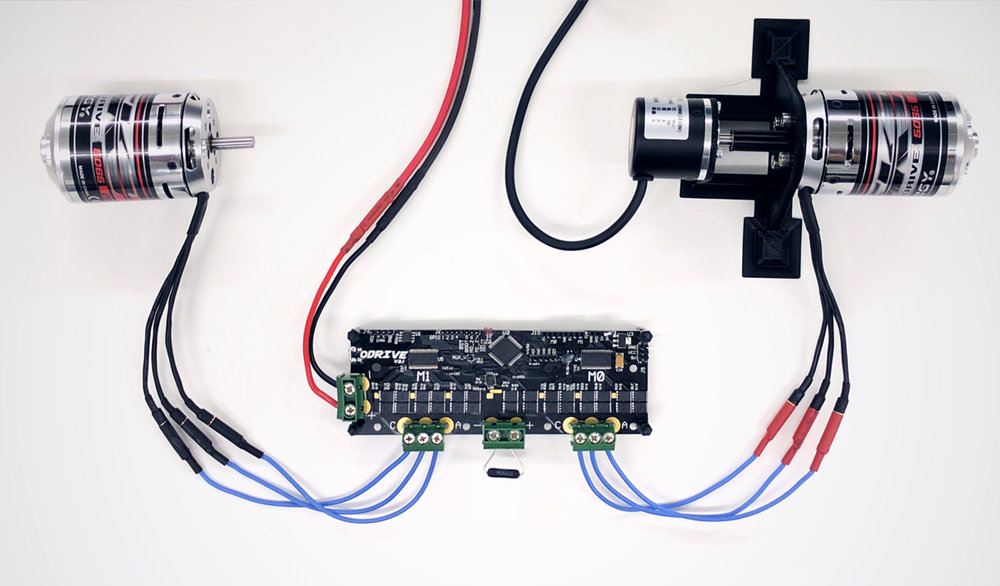
\includegraphics[width=0.6\textwidth]{Odrive.jpg}
\caption{Odrive setup\cite{Odrive}}
\end{figure}


\chapter{System Design}
\vspace{-3mm}
The project was broken up into multiple stages, of which lead up to the design and manufacture of a PCB. This was used to create a list of goals that were required to be completed in order to successfully complete the project. This is also used to track the project progress in order to ensure that each stage of the project is accomplished in a timely manner.

\vspace{4mm}
\textbf{The project stages were:}
\begin{figure}[H]
\Centering
\begin{tabular}{l}
    1. Requirement Specification\\
    2. Design\\
    3. Component Testing\\
    4. Software\\
    5. PCB Design\\
    6. PCB Testing and Assembly\\
    7. Project Review\\
\end{tabular}
\end{figure}
\vspace{-7mm}
    
\section{Requirement specification}
The designed servomotor control board will need to have the following capabilities in order for it to be able to achieve the same functionality that devices such as the Dynamixel and other actuators can achieve. 

\vspace{7mm}
\textbf{The following functionality is required:}
\begin{table}[H]
    \centering
    \begin{tabular}{|c |c| c|}
    \hline
        \textbf{\underline{Control}} & \textbf{\underline{Communication}} & \textbf{\underline{Sensors}}\\
        Position  & UART  & Current\\
        Current & & Temperature\\
        \hline
    \end{tabular}
\end{table}
\newpage
\section{Hardware Design}
\vspace{-3mm}
An initial board layout based on the design specifications and requirements was created seen in Figure 3.1. This was used to determine all necessary components that would required. This is then also used when positioning the different components on the PCB.
\begin{figure}[H]
\centering
 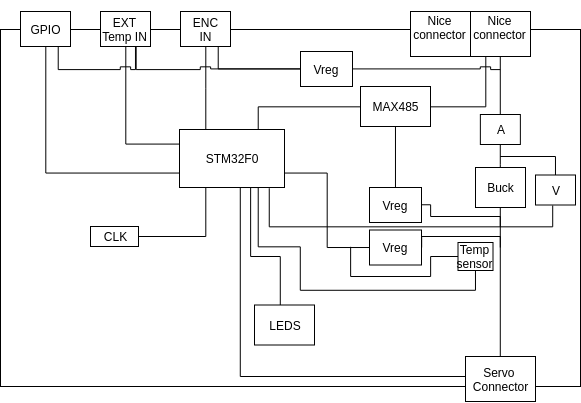
\includegraphics[width=0.58\textwidth]{My_board.png}
\caption{Basic board design}
\end{figure}  
\vspace{-7mm}
A flow diagram representing the two aspects of the system, power and communication can be seen in Figure 3.2.
\vspace{-2mm}
\begin{figure}[H]
\centering
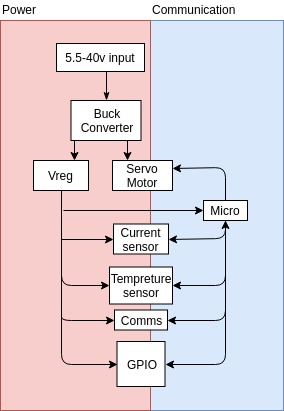
\includegraphics[width=0.45\textwidth]{System_Flow.jpg}
\caption{System flow diagram}
\label{fig:sysflow}
\end{figure}

\newpage
\section{Software Design}
The Slave microcontrollers will be programmed to interact with all its peripherals and perform communication using standard protocols. The Master microcontroller will control each Slave and be able to request information such as temperature and current drawn. A basic diagram of the interaction between the microcontroller and the code running on them can be seen in Figure 3.3.

\begin{figure}[H]
\centering
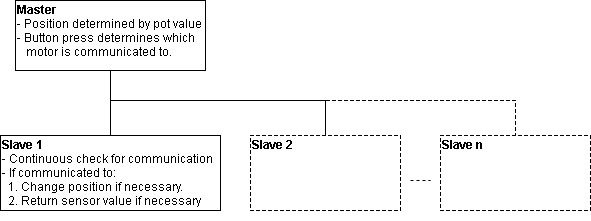
\includegraphics[width=0.9\textwidth]{Master_slave.jpg}
\caption{Master and Slave configuration}
\label{fig:masterslave}
\end{figure} 



\begin{figure}[H]
  \centering
  \begin{minipage}[b]{0.45\textwidth}
    \subsection{Master logic}
    The logic for the code running on master microcontroller can be seen in the diagram below in Figure 3.4.
    \vspace{2mm}
    \begin{figure}[H]
    \centering
    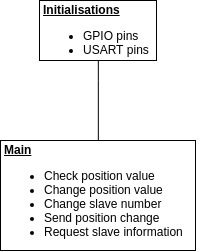
\includegraphics[width=0.8\textwidth]{Master_flow.jpg}
    \caption{Master code flow}
    \label{fig:MASTERFLOW}
    \end{figure} 
  \end{minipage}
  \hfill
  \begin{minipage}[b]{0.45\textwidth}
    \subsection{Slave logic}
    The logic for the code running on the slave microcontrollers can be seen in the flow diagram below in Figure 3.5.
    \vspace{5mm}
    \begin{figure}[H]
    \centering
    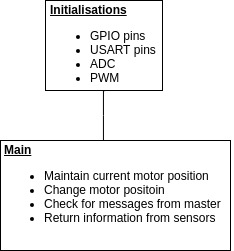
\includegraphics[width=0.9\textwidth]{Slave_flow.jpg}
    \caption{Slave code flow}
    \label{fig:SLAVEFLOW}
    \end{figure} 
  \end{minipage}
\end{figure}
\vspace{-5mm}

\newpage
\section{Component Selection}
After the system requirements have been established, and a basic system design has been created. The necessary components can be chosen.

The components that were chosen for the board had to be small enough to make the board compact, but still big enough so that it could be soldered down by hand accurately. Ideally a pick and place machine could be used to do the soldering, allowing for smaller components to be chosen, but for the sake of producing a functioning prototype it was only practical to choose slightly bigger components.


\subsection{Microcontroller}
The chosen micro controller needed to have the ability to interact with all the peripherals on the board as well as complete necessary computations in order for it to be able to control the servo motor board. As well as meeting the technical specifications, the chosen micro needed to be well documented in order to simplify the coding and debugging process.

The STM32F051C6 has an ARM Cortex-32-bit RISC core operating at up to 48MHz. This microcontroller was chosen as it met all the requirements and includes the following peripherals and functionality:
\vspace{5mm}
\begin{table}[H]
\centering
    \begin{tabular}{|c|c|}
    \hline
      \textbf{\underline{Features}} & \textbf{\underline{Types of communication}}\\
      64Kbytes of Flash & I2C \\
      12 bit ADC & SPI\\
      12-bit DAC & I2S\\
      six 16-bit timers & HDMI\\
      32-bit timer & USART\\
      Advanced control timer & \\
      Temperature sensor & \\
      \hline
    \end{tabular}
\end{table}
\vspace{-5mm}
The STM32F051C6 supports hardware controlled RS485 USART communication which will allow for the communication between the micro controllers using the MAX485 chip.
Its 12-bit ADC is a successive approximation analogue-to-digital converter. 

\newpage 
\vspace{5mm}
It has up to 16 channels which can be used to read the output voltage from the current and temperature sensors as well as from other GPIO pins. A 16-bit timer will be used to output the PWM signal the will be used to control the servomotors position.With multiple low power modes minimising the overall power consumption, optimising performance and consumption which is very important for applications that are run off batteries. 

\vspace{7mm}
In Figure 3.6, the necessary net labels were appended to the pins that are required for the microcontroller to function, as well as the pins that will be used to interact with the different peripherals.\vspace{2mm}
\vspace{10mm}
\begin{figure}[H]
\centering
\vspace{-5mm}
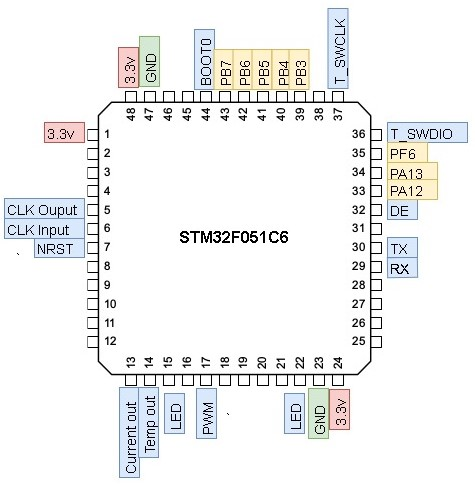
\includegraphics[width=0.6\textwidth]{micro.jpg}
\caption{STM32F051 LQFP48 package\cite{STM}}
\label{fig:STM}
\end{figure}
\vspace{1mm}
The STM will be programmed using the Atollic TrueSTUDIO IDE. The code was then compiled to hardware code and uploaded to the microcontroller using the ST-link debugger supported by Atollic.

\newpage
\subsection{Temperature sensor}
\vspace{5mm}
An analogue temperature sensor was chosen, the voltage output will be connected to one of the microcontrollers ADC. The MCP9700T has been designed for general purpose temperature monitoring and is typically used in home appliance and office equipment as well as hard disks and other PC peripherals.
\vspace{2mm}
\begin{figure}[H]
  \centering
  \begin{minipage}[b]{0.4\textwidth}
    \centering
    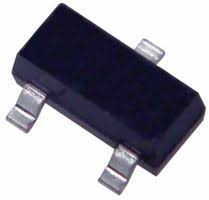
\includegraphics[width=0.4\textwidth]{MCP9700T.jpeg}
    \caption{MCP9700T chip \cite{MCP9700T} }
  \end{minipage}
  \hfill
  \begin{minipage}[b]{0.55\textwidth}
    \begin{table}[H]
      \centering
        \begin{tabular}{|l|}
        \hline
          \textbf{The MCP9700 has the following features:}\\
            - Input voltage range of 2.3V to 5.5V\\
            - Operates between -40\degree C to 125\degree C\\
            - 2\degree C accuracy between 0\degree C to 70\degree C\\
            - 10.0mV/\degree C resolution\\
            \hline
        \end{tabular}
        \caption{MCP9700 features}
    \end{table}
  \end{minipage}
\end{figure}
Unlike resistive sensors, the Linear Active Thermistor IC does not require any signal conditioning and the Vout pin should be directly connected to the input of a microcontroller.
The temperature coefficients are scaled to provide a 1\degree C/bit resolution for an 8-bit ADC with a reference voltage of 2.5V and 5V respectively.
This device is immune to the effects of parasitic capacitances which provides flexibility with the PCB layout as the device can be remotely located from the micro controller.

\begin{figure}[H]
  \centering
    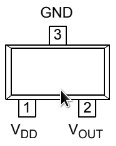
\includegraphics[width=0.15\textwidth]{MCP9700_setup.png}
    \caption{MCP9700 typical setup}
    \label{fig:model}
\end{figure}


\newpage
\subsection{Current sensor}
The chosen current sensor was the INA169 high side current shunt monitor. It is an analogue current sensor that produces and output current relative to that of a differential input voltage. The input voltage is read from either side of a current sensing resistor RS. The output current is then converted to a voltage across a load resistor RL. The voltage gain depends on the size of the Rl and thus can be controlled to have an output voltage of the same range as the input to the microcontrollers ADC. As a result the output can be connect directly to the input of the microcontroller ADC.

This type of  current sensor is typically used in automotive, computer and cellphone power management amongst other things. 
\begin{figure}[H]
  \centering
  \begin{minipage}[b]{0.4\textwidth}
    \centering
    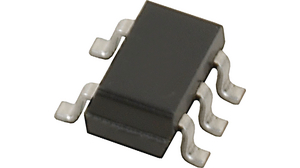
\includegraphics[width=0.5\textwidth]{INA169.jpg}
    \caption{INA169 chip \cite{INA169} }
  \end{minipage}
  \hfill
  \begin{minipage}[b]{0.55\textwidth}
    \begin{table}[H]
    \centering
        \begin{tabular}{|l|}
        \hline
        \textbf{The INA169 has the following features:}\\
            - Input voltage range of 2.7V -60 V\\
            - Functions normally from -40\degree C to 85\degree C\\
            - A single resistor sets the gain.\\
            \hline
        \end{tabular}
    \caption{INA169 features}
    \end{table}
  \end{minipage}
\end{figure}
\vspace{-5mm}
The typical current sensor configuration can be seen below in Figure 3.10 with $RL = 10k\ohm$ and $RS = 0.1\ohm$. This gives the current sensor the ability to accurately sense voltage in the range of 350mA-3.5mA which is what can be required from the servo motor at higher loads. A 0.1uF capacitor is recommended between the V+ input and ground. The INA169 can be set up with different values of Rs in order to measure different current ranges. The different resistances associated with the different current ranges can be seen in the table below \cite{Rs_range}.
\vspace{-2mm}
\begin{figure}[H]
  \centering
  \begin{minipage}[b]{0.45\textwidth}
    \begin{figure}[H]
        \centering
        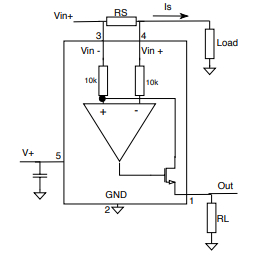
\includegraphics[width=0.65\textwidth]{INA169_setup.jpg}
        \vspace{-5mm}
        \caption{INA169 configuration}
        \label{fig:currentsense}
    \end{figure}
  \end{minipage}
  \hfill
  \begin{minipage}[b]{0.45\textwidth}
    \begin{table}[H]
    \centering
    \begin{tabular}{|c|c|}
    \hline
        \textbf{Rs} & \textbf{Range}\\
        10\ohm  & 3.5mA-35mA\\
        1\ohm   & 35mA-350mA\\
        0.1\ohm & 350mA-3.5A\\
        \hline
    \end{tabular}
    \vspace{5mm}
    \caption{Current sense range.}
    \end{table}
  \end{minipage}
\end{figure}


\newpage
\subsection{MAX485}
The MAX485 is a low power level shifting RS485 transceiver chip which operates from a single 5V supply. The IC contains one driver and one receiver. The receiver has an input has a fail-safe feature that guarantees a logic-high output if the input is open circuit.
\vspace{2mm}

\begin{figure}[H]
  \centering
  \begin{minipage}[b]{0.38\textwidth}
    \centering
      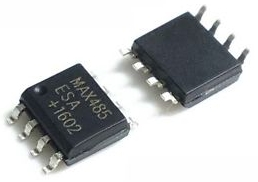
\includegraphics[width=0.6\textwidth]{max485.jpg}
    \caption{MAX485 chip \cite{max485} }
  \end{minipage}
  \hfill
  \begin{minipage}[b]{0.59\textwidth}
    \begin{table}[H]
    \centering
    \begin{figure}[H]
        \centering
        \begin{tabular}{|l|}
        \hline
        \textbf{The MAX485 has the following features:}\\
        - Common-Mode input voltage range from -7V to 12V\\
        - Functions normally from 0°C to 70°\\
        - Allows for up to 32 transceivers on the bus\\
        - Has a data rate of 2.5Mbps\\
        - Current-limiting shutdown protection\\
        - Thermal shutdown protection\\
        \hline
        \end{tabular}
    \end{figure}
    \end{table}
  \end{minipage}
\end{figure}

The data sheet supplies all the information required to run the MAX485 chip, this was used to create the pin setup seen below in Figure 3.12. Which was used when creating the testing methods.
\vspace{15mm}

\begin{figure}[H]
\centering
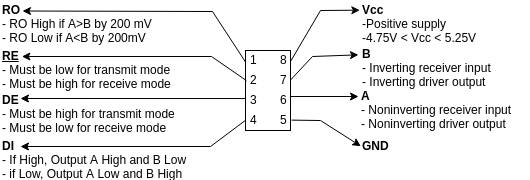
\includegraphics[width=1\textwidth]{MAX485_setup.png}
\caption{MAX485 pin setup}
\label{fig:model}
\end{figure}

\newpage
\subsection{Communication lines}
\vspace{-5mm}
The connector cable used for the communication will be constructed from two wires that twist together over the length of the connection and terminated with termination resistors between the two cables at the beginning and end of each connection. The twisting of the wires is done for the purpose of cancelling out any electromagnetic interference from any external source as well as any noise produced from switch mode power supplies nearby\cite{twisted}.

\vspace{-5mm}
\begin{figure}[H]
\centering
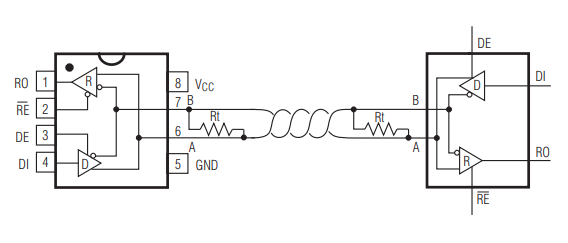
\includegraphics[width=0.6\textwidth]{MAX485_example.png}
\vspace{-7mm}
\caption{Differential communication over the twisted pair \cite{twistedpair}}
\end{figure} 
\vspace{-8mm}
Termination resistors, Rt, are used to match the impedance of a transmission line to the hardware impedance of the interface it is connected to. This allows the the signals to be received with maximum power.  Unterminated, or termination with some value unequal to the impedance of the cable, leads to mismatch that creates reflections in the network. Reflections are part of the energy of the signal that literally returns back up the line. Reflections can constructively or destructively interfere with the next bits propagating down the bus\cite{termination}.

\vspace{-7mm}
\subsection{Connector}
\vspace{-5mm}
The chosen connectors for the servo board had different requirements. The connectors from the buck converter to the servo motor needed to be able the high currents that the motor could draw while the rest of the pins will be used for low current applications. For this, the Molex through hole male pin connectors were chosen which can handle up to 4A.
\vspace{-5mm}
\begin{figure}[H]
\centering
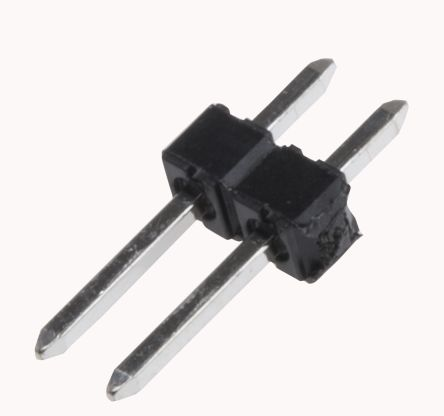
\includegraphics[width=0.3\textwidth]{molex.jpg}
\caption{Molex though hole male pin connector\cite{molex}}
\label{fig:model}
\end{figure} 
\vspace{-5mm}


\newpage
\subsection{Buck Converter}
\vspace{-3mm}
The buck converter chosen for this design needed to output 5V at up to 4 A, with an input voltage range of 5.5-40 Volts. While being small enough to minimise space but big so that it can be still soldered by hand. Using Texas Instruments online power supply designer, Webench. Webench generates the required circuit component values when choosing a buck converter. There were four options where available, seen below in Table 3.4.
\begin{table}[H]
    \centering
    \begin{tabular}{|l|}
    \hline
        1. LM5088 HTSSOP (16 pin) 5.00 mm × 4.00 mm package\\
        2. TPS54561  WSON (10 pin) a 4.00 mm × 4.00 mm package\\
        3. TPS54560 HSOP (8 pin) 4.89 mm x 3.9 mm package\\
        4. LM5145RGYR VQFN (20 pin) 3.50 mm × 4.50 mm  package\\
        \hline
    \end{tabular}
    \caption{Available buck converters}
\end{table}
\vspace{-5mm}
The buck converter chosen was The LM5088, a high voltage non-synchronous buck controller which features all the necessary functions to implement an efficient high voltage buck converter using a minimum number of external components. This Buck controller is typically used for motor driver and USB powered applications. 
\vspace{-2mm}
\begin{figure}[H]
  \centering
  \begin{minipage}[b]{0.4\textwidth}
    \centering
        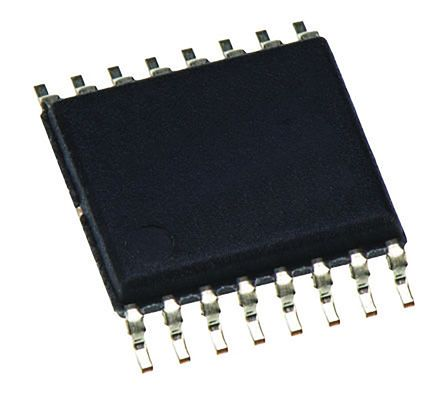
\includegraphics[width=0.45\textwidth]{buck.jpg}
        \caption{LM5088 \cite{buck}}
        \label{fig:model}
  \end{minipage}
  \hfill
  \begin{minipage}[b]{0.55\textwidth}
    \begin{table}[H]
      \centering
        \begin{tabular}{|l|}
        \hline
          \textbf{The LM5088 has the following features:}\\
            - Operates between -40\degree C to 125\degree C\\
            - Input voltage range of 4.5V to 75V\\
            - Thermal shutdown protection\\
            - Adjustable output voltage from 1.205V\\
        \hline
        \end{tabular}
        \caption{LM5088 features}
    \end{table}
  \end{minipage}
\end{figure}
\vspace{-4mm}
A simplified schematic of the typical setup of the LM5088 with all its needed external components can be seen below in Figure 3.16.
\begin{figure}[H]
  \centering
    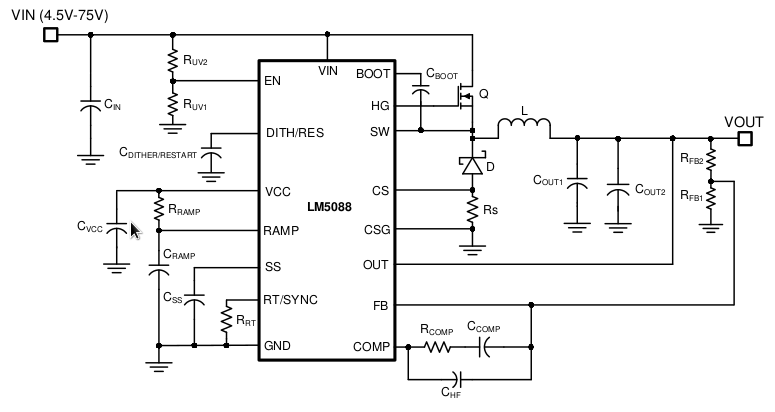
\includegraphics[width=0.6\textwidth]{LM5088_setup.png}
    \caption{LM5088 typical setup}
\end{figure}




\newpage
\subsection{Voltage regulator}
\vspace{4mm}
The voltage regulator chosen needed to be able to regulate the 5V output from the buck converter to the 3.3V needed by the microcontroller to run. The MCP1702 chip is a low power compact chip that only requires an input and output capacitor to run. 
\vspace{4mm}
\begin{figure}[H]
  \centering
  \begin{minipage}[b]{0.4\textwidth}
    \centering
    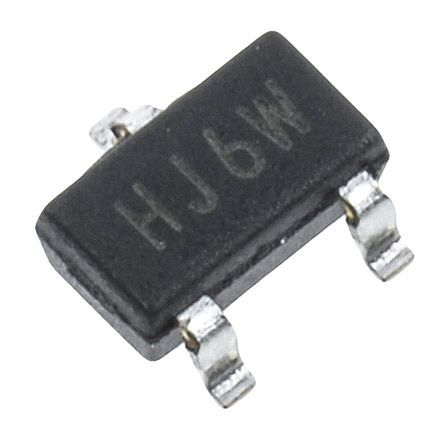
\includegraphics[width=0.4\textwidth]{MCP1702.jpg}
    \caption{MCP1702 chip}
  \end{minipage}
  \hfill
  \begin{minipage}[b]{0.55\textwidth}
    \begin{table}[H]
      \centering
        \begin{tabular}{|l|}
        \hline
          \textbf{The MCP1702 has the following features:}\\
            - Input voltage range of 2.7V to 13.2V\\
            - Output 3.3V with a 0.4\%  tolerance\\
            - Short circuit protection\\
            - Thermal shutdown protection\\
            \hline
        \end{tabular}
        \caption{MCP1702 features}
    \end{table}
  \end{minipage}
\end{figure}
\vspace{5mm}
The MCP1702 is a low dropout (LDO) voltage regulator. Typically used in battery powered applications, smoke detectors as well as digital cameras amongst other devices and applications.
\vspace{5mm}
A simplified schematic of the typical setup of the MCP1702:
\begin{figure}[H]
  \centering
    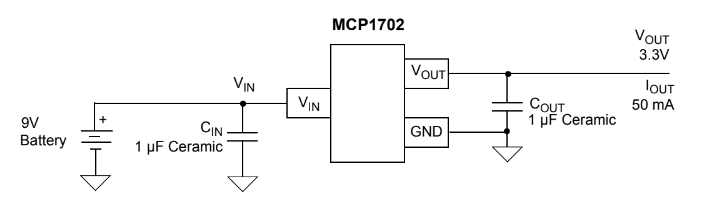
\includegraphics[width=0.8\textwidth]{MCP1702_setup.png}
    \caption{MCP1702 typical setup}
    \label{fig:model}
\end{figure}










 




 

\chapter{Component Testing}
\vspace{-12mm}
The components chosen where all Surface-Mount Devices (SMD) in order to minimise the size of the designed PCB. In order to test these components, they were soldered onto pieces of Vero board with male headers so the the component can be connected to a bread board for testing. Any code that was used has been included in the testing procedure and schematics are available in the GitHub repository.

\vspace{-4mm}
\section{Microcontroller} 
\vspace{-4mm}
To test the basic functioning of the micro controller, a schematic was designed with the minimum components required to run the microcontroller and allow for a simple test. The microcontroller will simply turn an LED on and off every 100 mili seconds. This was then implemented on a bread board.

The designed schematic included the necessary components required to run the micro controller. This included an 8MHz external clock, a reset push button, GPIO and debugger pins as well as an LED indicator. As well as the USB debugger setup.

\subsection*{Implemented code:}
\vspace{4mm}
\begin{table}[H]    
    \Centering
    \begin{tabular}{|l|l|}
    \hline
    \textbf{Initialisations:}&\textbf{Main:}\newline\\
    \vspace{-2mm}
    1. GPIO pins for LED's & 1. LED on\\
                           & 2. 100ms delay\\
                           & 3. LED off\\
                           & 4. Item 100ms delay\\
                           \hline
    \end{tabular}
    \caption{Microcontroller code implementation}
\end{table}
    


 



\newpage
\section{Temperature Sensor}
In order to test the temperature sensor. A test would need to be created where the sensors output voltage can be measured and related to the temperature. This test requires that the temperature sensor used for the reference has been calibrated. The reference sensor and the sensor being tested would then be exposed to various temperatures and the results will be tabulated and the sensed temperature can then be calculated using the fact that the sensor output 500mV at 0\degree C, found in the datas heet .Thus at 25\degree C, the Temperature$\mathbf{ = \frac{Vout - 500mV}{gain}}$.

An alcohol thermometer was used as the reference temperature sensor. The thermometer was calibrated by submerging it in an ice bath and reading the temperature after five minutes. The thermometer read 0\degree C, the temperature of ice melting, which meant it was calibrated.

The device was connected following the schematic, but no other components are necessary to run the device. It is suggested in the data sheet to connected a 0.1uF capacitor between $V_D $ and Ground and the gain was set to 10 by using RS = 10\ohm. The chip was then exposed to multiple temperatures while recording Vout using an oscilloscope. Vout was then measured and the actual and sensed temperatures were tabulated below in Table 4.2.
\vspace{5mm}
\begin{table}[H]
\centering
    \begin{tabular}{|c| c| c|}
    \hline
     \textbf{\underline{Actual Temperature (\degree C)}}  & \textbf{\underline{Vout (V})} & \textbf{\underline{Sensed Temperature(\degree C)}}\\
     25 & 0.738 & 23.8 \\
     28 & 0.775 & 27.5 \\
     50 & 0.984 & 48.4 \\
     62 & 1.098 & 59.8 \\
     68 & 1.11  & 61.0 \\
     87 & 1.25  & 75.0 \\
     \hline
    \end{tabular}
    \caption{Temperature sensor results}
\end{table}
The temperature sensor worked with expected accuracy. The MCP1700 data sheet specifies a 2\degree C error for temperatures less than 55\degree C. This accuracy can be seen between 25\degree C-50\degree C. For the results above 55\degree C it can be seen that as the variance increases as the temperature increases.


\newpage
\section{Current Sensor}  
\vspace{-7mm}
In order to create a stable current source for the current sensor, A resitor bank is used for the load. This will allow for the resistance to be changed incrementally by connecting at different points along the resistor bank. Along with a known resistance, applying a constant 10V across the output load will allow for the current through Rs to be known and easily controllable. The INA169 was in its standard configuration. RL was chosen to be 10k\ohm for a gain of 10. For testing purpose a current range of 1mA - 30mA would be tested for and an Rs of 10\ohm. This will allow for sensing at this current range. A lower current range was chosen for testing as low currents are safer and is cheaper to work with. When creating the resistive load bank, it had to be taken note of that the max differential voltage that can be experienced between Vin+ and Vin- is 500mV which outputs an Iout of 500uA. This required that the load needed to have a resistance greater than at least 10 times more than that of the sensing resistor RS.

\vspace{-3mm}
The actual drawn current was simply calculated using $V=IR$. The current measured by the sensor was calculated using $Is =  \frac{Vout*1k\ohm }{10*10k\ohm}$. The output current, voltage and sensed current equations were found in the data sheet.
\vspace{-5mm}
\begin{itemize}
    \item[] $\mathbf{Iout = gm(Vin+ - Vin-)}$, \hspace{10mm} $\mathbf{gm = 1000\frac{uA}{V}}$
    \item[] $ \mathbf{Vout = \frac{Is*Rs*Rl}{1k\ohm}}$  \hspace{33mm} $ \mathbf{Is = \frac{Vout*1k\ohm}{Rs*Rl}}$
\end{itemize}

\vspace{-5mm}
Table 4.3 shows the input and output, as well as the actual and calculated current values that were recorded during the testing. The load resistance in the table refers to the output load being used to create a specific current, not to be confused with RL the load resistor that determines the gain for Vout.

\begin{table}[H]
\centering
    \begin{tabular}{|c| c| c| c|}
    \hline
     \textbf{\underline{Load resistance (\ohm)}}  & \textbf{\underline{Iactual (mA)}} & \textbf{\underline{Vout (V)}} & \textbf{\underline{Is (mA)}}\\
     900 & 10 & 0.98 & 9.8  \\
     800 & 12 & 1.12 & 11.2 \\
     700 & 14 & 1.28 & 12.8 \\
     600 & 16 & 1.47 & 14.7 \\
     500 & 18 & 1.74 & 17.4 \\
     400 & 24 & 2.2  & 22   \\
     300 & 30 & 2.8  & 28   \\
     \hline
    \end{tabular}
     \caption{Current sensor results}
\end{table}
\vspace{-9mm}
The current sensor was able to sense and calculate the output current with an error of about $+- 2mA$. It was found that at resistances of less than 400\ohm  the fraction of the voltage drop across Rs relative to the voltage drop across the load becomes big enough for it to effect the sensed current Is, resulting in a less accurate Vout voltage.

\newpage
\section{MAX485}
\vspace{-8mm}
Termination resistors of RT = 120\ohm for RS485 communication when impedance matching and a 1uF capacitor between $V_{cc}$ and ground for to stabilising the voltage ripple. The MAX485 chip can be tested in its two states, transmitting and receiving. 

\begin{table}[H]
\centering
    \begin{tabular}{|l|l|}
    \hline
            \textbf{\underline{Transmitting:}}&\textbf{\underline{Receiving:}}\\
            1. Connect chip to ground and power          & 1. Connect power and ground\\
            2. Connect \underline{RE} to ground          & 2. Write data to USART TDR\\
            3. Connect DE to 5V                          & 3. Connect \underline{RE} to 5V\\
            4. Supply DI with a PWM signal               & 4. Supply DI with a PWM signal\\
            5. Use oscilloscope to probe pins A and B    & 5. Differential signal is applied to pins A and B\\
                                                         & 6. Use oscilloscope to probe pins RO \\
                                  \hline
    \end{tabular}\
    \vspace{-3mm}
    \caption{Transmission and reception tests}
    \vspace{-13mm}
\end{table}

\subsection{Implementation}
\vspace{-7mm}
When testing the MAX485 the transmission and reception test were both successful indicating a correct setup of the transceiver. The oscilloscope readings of both the transmission and reception tests can be seen below in Figures 4.1-4.4.

\vspace{-1mm}
\begin{table}[H]
    \centering
    \begin{tabular}{|c|c|}
    \hline
    \textbf{\underline{Transmission test}}&\\
    \vspace{-5mm}
      \begin{minipage}[b]{0.45\textwidth}
        \begin{figure}[H]
            \centering
            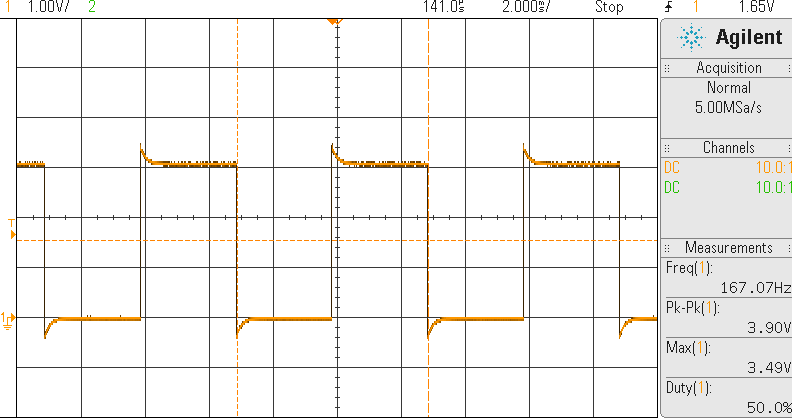
\includegraphics[width=1\textwidth]{max_trans_signal.png}
            \vspace{-8mm}
            \caption{\small{Signal to be transmitted}}
        \end{figure}
      \end{minipage}
       &   
      \begin{minipage}[b]{0.45\textwidth}
        \begin{figure}[H]
            \centering
            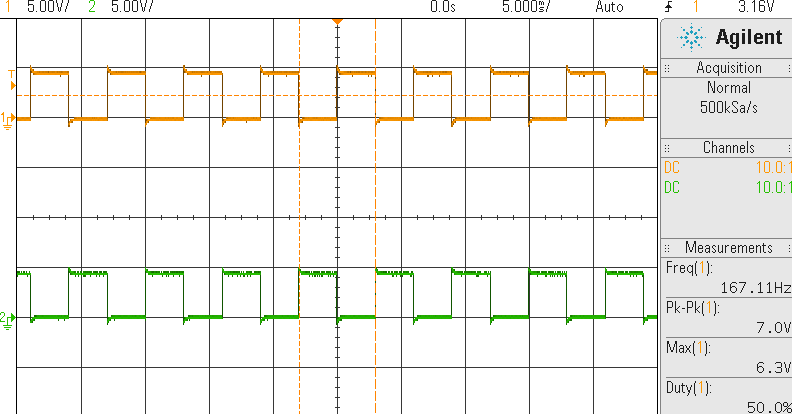
\includegraphics[width=1\textwidth]{max_trans_outputAB.png}
            \vspace{-8mm}
            \caption{\small{A and B output transmitted}}
        \end{figure}
      \end{minipage}\\
      &\\
      \hline
    \textbf{\underline{{Reception test}}} & \\
    \vspace{-5mm}
    \begin{minipage}[b]{0.45\textwidth}
    \begin{figure}[H]
        \centering
        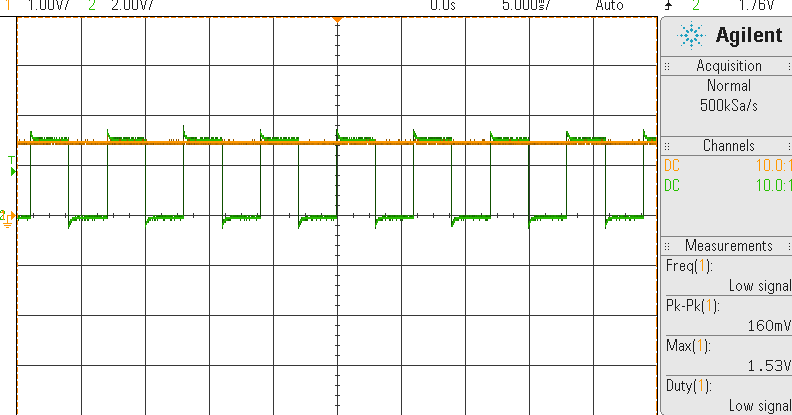
\includegraphics[width=1\textwidth]{max_recieve_signal.png}
        \vspace{-8mm}
        \caption{\small {Signal being received}}
    \end{figure}
    \end{minipage}
    &
    \begin{minipage}[b]{0.45\textwidth}
    \begin{figure}[H]
        \centering
        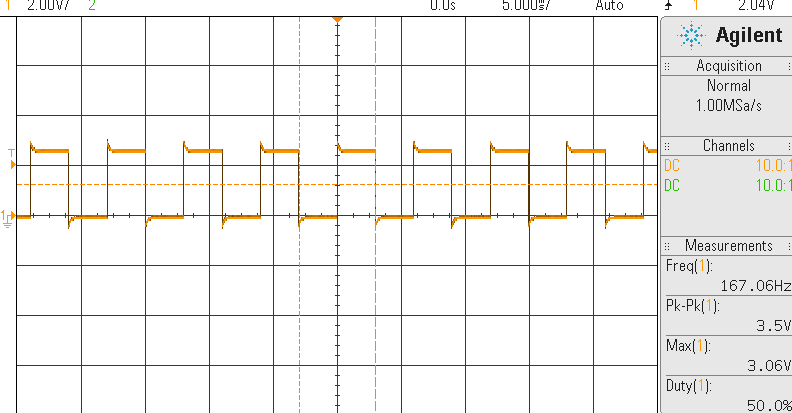
\includegraphics[width=1\textwidth]{max_receive_output.png}
        \vspace{-8mm}
        \caption{\small{RO received signal}}
    \end{figure}
    \end{minipage}\\
    &\\
    \hline
    \end{tabular}
    \caption{Caption}
\end{table}
\vspace{-5mm}




\newpage
\section{Buck Converter}
The data sheet for the LM5088 includes a typical setup for this particular buck converter. It goes through each step in the design procedure as well as all the equations needed to solve for all the necessary resistor and capacitor values as well as any other needed components that are required to run the buck converter.

Texas Instruments online power supply designer, WeBench was used to choose the buck converter chip and components required to produce the required output voltage.

The chosen buck converter design consisted of only surface mount components. The buck converter chip has a thermal pad at its base and with 16 pins it made it impossible to assemble the buck converter for testing.

Though it can be assumed that the designed buck converter works as Texas Instruments is reliable supplier of electronic equipment and components.




\newpage
\section{Voltage Regulator}
The MCP9700 chip was connected to 5V and Ground. The output voltage was then measured at the output pin. 

The regulator stability was then tested for various current draws using a resistor bank as a load. The results can be seen below in Table 4.6.

\begin{table}[H]
\centering
    \begin{tabular}{|c| c| c|}
    \hline
    \textbf{\underline{Load resistance (\ohm)}}  & \textbf{\underline{$I_{out}$ (mA)}} & \textbf{\underline{Vout (V)}}\\
       1k\ohm   & 3.3  & 3.28\\
       500\ohm  & 6.6  & 3.32\\
       250\ohm  & 13.2 & 3.35\\
       200\ohm  & 16.5 & 3.33\\
       125\ohm  & 26.4 & 3.37\\
       100\ohm  & 33   & 3.38\\
   \hline
    \end{tabular}
    \caption{Voltage load stability}
\end{table}
Various input voltages were applied in order to test the stability of $V_{OUT}$ with a constant load. The results can be seen below in Table 4.7.

\begin{table}[H]
\centering
    \begin{tabular}{|c| c|}
    \hline
      \textbf{\underline{$V_{IN}$}}  & \textbf{\underline{Vout (V)}}\\
       2 & 2.2  \\
       3 & 2.8 \\
       4 & 3.35\\
       5 & 3.33\\
       6 & 3.37\\
       7 & 3.32\\
       8 & 3.28\\
      \hline
    \end{tabular}
    \caption{Voltage stability}
\end{table}
It was found that the voltage regulator functioned well for voltages above 2.5V and maintained a stable output voltage regardless of the change in input voltage.
\chapter{PCB Design}
Once the components were chosen and there schematics drawn up. Altium Designer was then used to create the PCB design of the servo motor controller that could then be converted into a format that the PCB manufacturers, TraX, can then use to create the PCB. The board was designed in several stages.

\section{Schematic}
The first step in designing the PCB on was to create each of the designed schematics in Altium. All the necessary pins, net labels were connected up for each component. The schematics can be seen in the following pages.
\begin{figure}[H]
\centering
\includegraphics[width=1\textwidth]{Microsch.jpg}
\vspace{-5mm}
\caption{Microcontroller and components schematic}
\end{figure} 

\newpage
\begin{figure}[H]
\centering
\includegraphics[width=0.85\textwidth]{bucksch.jpg}
\caption{Buck converter schematic}
\end{figure} 

\newpage
\section{Parts and footprints}
Each component chosen will have an associated PCB footprint, where the solder pads and through connectors may be soldered. Most resistors, capacitors and inductors come in various standard package sizes, but other components such as the MOSFET or buck converter will have their own unique footprint. For these components the parts and their footprints had to be specifically made using measurements from the associated data sheet. 

First each component needed to be designed in an Altium library. This is where the pin numbers and outputs are allocated. 
\hspace{5mm}
\begin{figure}[H]
\centering
\includegraphics[width=0.8\textwidth]{library.JPG}
\caption{Creating a component}
\label{fig:model}
\end{figure} 

Each components footprint was also then created. This is where the actual solder pad for each pin is created.
\hspace{5mm}
\begin{figure}[H]
\centering
\includegraphics[width=0.7\textwidth]{footprints.JPG}
\caption{Creating a footprint}
\label{fig:model}
\end{figure} 

\newpage
\section{Board optimisation}

Once the schematic was designed, and all the components and their footprints were either found in the free Altium libraries (Altium Vault) or created, a model of the PCB can be created. At this point the components can be placed and any physical specifications of the PCB can be defined. 

In an initial design, the placement of components and the routing of the tracks had been done in a messy and inefficient way.  The tracks created between components looped around other components or obstacles when attempting to take the shortest route. Laying tracks like this can lead to stray inductances, more importantly, the tracks between all the components were the same width and did not take current requirements into account which can lead to the tracks breaking and causing damage to the PCB. No ground plain had been used and this added to additional ground tracks running across the PCB. 

\vspace{-5mm}
\subsection{Track parameters}    
The buck converter will be supplying all the current to the servo motor as well as to the rest of the components on the board board. The standard track width automatically set on Altium Designer is 0.25mm, which is much too thin to carry up the 4 Amps that the buck converter was designed to output. Using the following formula the necessary trace width was calculated \cite{tracewidth}.
\vspace{-2mm}
\begin{center}
\Large
$ Width = \frac{(Current[Amps]/(k*(Temprise[\degree C]^b)^(1/c)))} {(Thickness[oz]*1.378[mils/oz]) }$

\begin{table}[H]
\centering
  \begin{tabular}{cl}
    \textbf{Where :}\\
    & k = 0.024 \\
    & b = 0.044\\
    & c = 0.725\\
    & Current  = 4 A\\
    & Temprise = 10 \degree C\\
    & Thickness = 0.725 mm\\
   
  \end{tabular}
\end{table}
\end{center}
\vspace{-5mm}
it was calculated that the track width would need to be roughly 2.8 mm, so a safe width of 4 mm was chosen for all the tracks that would be carrying high current. The lower current pins were given a track width of 0.8 mm.


\subsection{Component positioning}
\vspace{-5mm}
The buck converters positioning relative to the rest of the components, especially the microcontroller, is an important factor. Switch mode supplies tend to generate a switching noise at the switching frequency which is generally between 500kHz and 3MHz \cite{noise}. This was solved in two ways. First was to separate the buck converter from the microcontroller by putting the two devices on opposite sides of the board. The other  was to create a ground plane on the top and bottom of the board. The ground plane would would then ground any stray EM signals that will be created. This would also neaten up the board by reducing the number of ground tracks that would be otherwise required. This was achieved using Altium Designers Polygon pours option setting.

Once the buck converter had been placed, the next few parts that needed to be positioned were the current and temperature sensors, the 3.3v regulator, and the MAX485. All of these were relatively straight forward, keeping in mind that the MAX485 needed to be as close to the micro as possible as to reduce any possible noise. Any input and output pins as well as the reset button and any LED's were then positioned in such a way as to optimise the functioning of the board as well as to keep it as compact as possible.

\vspace{-5mm}
\subsubsection{Optimised layout}    
\vspace{-5mm}
The layout for the optimised PCB can be seen in Figure 3.18 with each individual components being highlighted.
\begin{figure}[H]
\centering
\includegraphics[width=0.6\textwidth]{PCB_breakdown.jpg}
\caption{Optimised PCB layout}
\end{figure} 
\vspace{-5mm}

\subsection{Final Design}
\vspace{-5mm}
The final schematic for the PCB design can be seen below in Figure 5.6. The top(red) and bottom(blue) layer tracks and pads can be seen. The top and bottom ground planes were removed for this schematic to make the tracks more visible.
\vspace{-2mm}
\begin{figure}[H]
\centering
\includegraphics[width=0.7\textwidth]{Final_PCB.jpg}
\caption{Final PCB design}
\end{figure} 
\vspace{-10mm}
Once the final design was completed it was exported to the Gerber format and sent of to Trax, where the actual PCB was manufactured.

\vspace{-10mm}
\subsection{Component List}
\begin{table}[H]
    \vspace{-5mm}
    \centering
    \scriptsize{
    \begin{tabular}{|l|l|l|l|l|l|}
         \hline
         \textbf{\underline{Buck converter}}& \underline{R101.82} & \textbf{\underline{Micro}}  & \underline{R65.66 }& \textbf{\underline{Current sensor}}&\underline{R38.88} \\
         $R_{rp}$ = 1M\ohm      &0.63&   $R_{M1}$ = 1k\ohm   &0.62&   $R_{RL}$ = 10k\ohm      &0.63\\
         $R_{t}$ = 10.7k\ohm    &0.64&   $R_{M2}$ = 150\ohm  &0.66&  $R_{RS}$ = 0.1\ohm      &4.85\\       
         $R_{V1}$ = 7.15k\ohm   &0.66&   $R_{M3}$ = 1k\ohm   &0.67&   SC = INA169             &33.40\\ 
         $R_{V2}$ = 49.9k\ohm   &0.73&                       &&                           &\\
         $R_{cp}$ = 27.4k\ohm   &0..85& $C_{MC1}$ = 10pF &2.35&  \textbf{\underline{Temperature sensor}}&\underline{R3.61}\\
         $R_{RSNS}$ = 20M\ohm   &0.68&   $C_{MC2}$ = 10pF    &2.35&   ST = MCP9700T           &3.61\\     
         $R_{fbt}$ = 5.1k\ohm   &0.68&                       &&                           &\\
         $R_{B1}$ = 150\ohm     &0.62&   uC = STM32F051C6    &35.17&   \textbf{\underline{RS485}}&\underline{R72.11}\\     
                                &&   8mHz crystal           &4.83&   COMS = MAX485           &72.11\\
         $C_{hf}$ = 20pF        &0.56&   LED                 &5.23&                           &\\   
         $C_{cp}$ = 2.2nF       &0.32&   SMD push button     &13.78& \textbf{\underline{Voltage regulator}} &\underline{R8.28}\\ 
         $C_{bt}$ = 27nF        &0.61&                      &&    V2 = MCP1700T       &8.28\\  
         $C_{o1}$ = 82uF        &5.23&                      &&                           &\\                                          
         $C_{o2}$ = 2.2uF       &1.53&                      &&                           &\\                                              
         D1 = VSSC520S-M3       &8.45&                      &&                           &\\   
         M1 = IPD50N10S3l16  &14.67&                       &&                           &\\                                          
         L1 = 10uH              &10.12&                       &&                           &\\    
         B1 = LM5088            &54.52&                       &&                           &\\  
         \hline
         \textbf{Total cost: R290.36}&&&&&\\
         \hline
    \end{tabular}}
    \caption{Component list}
\end{table}
\vspace{-10mm}


\chapter{PCB Assembly and Testing}
\vspace{-14mm}
The PCB would be assembled in sections.  All the components required to get a certain aspect of the PCB functioning would be soldered down and then that aspect will be tested. 

\vspace{-1mm}
\textbf{Components to be assembled :}
\begin{figure}[H]
        \begin{enumerate}
        \setlength{\itemsep}{-1.5mm}
        \item Buck converter
        \item Voltage regulator
        \item Temperature sensor
        \item Current sensor
        \item Microcontroller
        \item MAX48
    \end{enumerate}
\end{figure}

\vspace{-8mm}
The voltage regulator, MAX485, temperature and current sensor chips all had simple configurations and when tested worked as expected as seen in chapter 4, Component Testing. The microcontroller and buck converter required a more complicated setup. The two chips and the components necessary for their functioning can be see soldered down in Figure 6.1.

\vspace{2mm}
\begin{figure}[H]
\centering
\includegraphics[width=0.8\textwidth]{Soldered_PCB.jpg}
\vspace{-1mm}
\caption{Microcontroller and buck converter on PCB}
\end{figure} 
\vspace{-5mm}

\newpage
\section{Buck Converter}
\vspace{-3mm}
The buck converter chip and all necessary components required for it to function were soldered on to the board. Headers were soldered down enabling the power, ground and output cables to be to connected allowing testing. A couple issues came up when soldering the buck converter to the PCB.
\vspace{-5mm}
\begin{enumerate}
    \item The capacitor values designed for had were only available in the electrolytic packages. The through hole capacitors were soldered to the surface mount pads. 
    \vspace{-3mm}
    \begin{figure}[H]
      \centering
      \begin{minipage}[b]{0.45\textwidth}
        \begin{figure}[H]
            \centering
            \includegraphics[width=0.62\textwidth]{footprint_buckconverter.jpg}
            \caption{Buck converter footprints}
        \end{figure}
      \end{minipage}
      \hfill
      \begin{minipage}[b]{0.45\textwidth}
        \begin{figure}[H]
            \centering
            \includegraphics[width=0.7\textwidth]{Solder_capacitors.jpg}
            \caption{LM5088 soldered down}
        \end{figure}
      \end{minipage}
    \end{figure}
    
    \vspace{-5mm}
    \item The MOSFET footprint that was designed had been chosen for a  different MOSFET that was not available from suppliers. The pins of the new MOSFET were in a different order and a wire had to be soldered across the pad so that the in order to allow the MOSFET to be connected correctly. This can be seen in Figures 6.4 and 6.5.
    
    \begin{figure}[H]
      \centering
      \begin{minipage}[b]{0.5\textwidth}
        \begin{figure}[H]
            \centering
            \includegraphics[width=0.7\textwidth]{Solder_mosfet.jpg}
            \caption{Correcting MOSFET}
        \end{figure}
      \end{minipage}
      \hfill
      \begin{minipage}[b]{0.45\textwidth}
        \begin{figure}[H]
            \centering
            \includegraphics[width=0.6\textwidth]{Solder_mosfet2.jpg}
            \vspace{-3mm}
            \caption{MOSFET soldered down}
        \end{figure}
      \end{minipage}
    \end{figure}
    \vspace{-3mm}
    \item When designing the footprint, no solder mask was inserted between the pins of the buck chip. The result of this was when soldering, solder leaked over creating shorts, as well as letting pins getting close enough to arc. Seen in Figures 6.6 and 6.7.
    
    \begin{figure}[H]
      \centering
      \begin{minipage}[b]{0.5\textwidth}
        \begin{figure}[H]
            \centering
            \includegraphics[width=0.7\textwidth]{footprint_buck.jpg}
            \caption{LM5088 footprint}
        \end{figure}
      \end{minipage}
      \hfill
      \begin{minipage}[b]{0.45\textwidth}
        \begin{figure}[H]
            \centering
            \includegraphics[width=0.83\textwidth]{Solder_buck.jpg}
            \vspace{-3mm}
            \caption{LM5088 soldered down}
        \end{figure}
      \end{minipage}
    \end{figure}
\end{enumerate}


\section{Microcontroller}
\vspace{-5mm}
The STM chip, clock, an indicator LED and necessary resistors and capacitors were placed on the board. Headers were soldered down enabling the power, ground and debugging cables to be to connected. 

The same mistake that had been made in the buck converter footprint design was made for the microcontroller. When connected to power and ground, the pins would short stopping the circuit from working. This can be seen in Figures 6.8 and 6.9.

\vspace{-2mm}
\begin{figure}[H]
  \centering
  \begin{minipage}[b]{0.45\textwidth}
    \begin{figure}[H]
        \centering
        \includegraphics[width=0.7\textwidth]{footprint_micro.jpg}
        \caption{STM footprint}
    \end{figure}
  \end{minipage}
  \hfill
  \begin{minipage}[b]{0.45\textwidth}
    \begin{figure}[H]
        \centering
        \includegraphics[width=1\textwidth]{Solder_micro.jpg}
        \vspace{-2mm}
        \caption{STM soldered down}
    \end{figure}
  \end{minipage}
\end{figure}






\chapter{Software}
\vspace{-19mm}
The STM microcontroller has an ARM Cortex-32-bit RISC core that will be programmed in C using Atollic TrueSTUDIO. The IDE will compile and upload the code to the STM using the ST-link debugger and toolchain. All code can be found in the GitHub repository. \textbf{https://github.com/Marshmellowfellow/Thesis-Servocontroller-Board.git}
\vspace{-12mm}

\section{ADC}
\vspace{-8mm}

\begin{table}[H]
\centering
    \begin{tabular}{|l|l|}
    \hline
            \textbf{\underline{Initialisations:}}&\textbf{\underline{Main:}}\\
            1. Configure GPIO pins & 1. Select channel to sample\\
            2. Enable ADC clock    & 2. Activate ADC to be read\\
            3. Set ADC parameters  & 3. Start conversion\\
                                   & 4. Read in ADC value\\
                                  \hline
    \end{tabular}
    \caption{ADC code implementation}
\end{table}

\vspace{-12mm}
\subsection{Testing}
\vspace{-7mm}
In order to test the implementation of the ADC code a voltage in the range 0V-3V will be applied to the ADC pin of the micro controller. The ADC will sample with an 8-bit resolution. This will give $\mathbf{2^8 - 1 = 255}$ bits, giving a resolution of $\mathbf{\frac{3}{255}\frac{V}{Steps}}$ = $\mathbf{11.76\frac{mV}{step}}$. 
\vspace{-9mm}

The ADC will store an 8-bit value representing the sampled input into the ADC Data Register(DR). This value will then be written to the General Purpose Input Output(GPIO) Output Data Register(ODR). GPIO pins 0-7 will be set in output mode and connected to an LED. The binary value of the sample can then be output to the 8-bit LED output so that it can be read and compared to the actual voltage at the ADC input pin. 

\vspace{-2mm}
The binary value output will be a number between 0-255. The voltage calculated using $V_{calculated} = (ADC_{output})\times(resolution) $. The applied voltages and sampled values can be seen below in ..table.. and were calculates using the resolution of $11.76\frac{mV}{step}$ 

\begin{table}[H]
\vspace{-2mm}
    \centering
    \begin{tabular}{ |c| c| c| }
        \hline
         \textbf{\underline{$\mathbf{V_{Applied}}$} (V)} & \textbf{\underline{Output 8-bit value}} & \textbf{\underline{$V{Calculated}$ (V)}} \\
         0.66 & 00110000 & 564.48 \\
         1.21 & 01011000 & 1.03 \\
         1.81 & 10000100 & 1.55 \\
         2.36 & 10101100 & 2.02 \\
         3.30 & 11111110 & 2.99 \\
         \hline
    \end{tabular}
    \vspace{-2mm}
    \caption{ADC testing applied voltages}
    \vspace{-3mm}
\end{table}
\vspace{-8mm}
It can be seen that with some error, the ADC was cable of sampling a voltage. Thus the microcontroller can read an output voltage from the current and temperature sensors.


\newpage
\section{PWM}
\vspace{-3mm}
The following configurations were implemented in order to output a PWM signal at a GPIO pin.

\begin{table}[H]
\centering
    \begin{tabular}{|l|l|}
    \hline
            \textbf{\underline{Initialisations:}}&\\
            1. Enable the GPIO clock        & 6. Set timer to PWM mode 1\\
            2. Enable the timer             & 7. Set signal frequency\\
            3. Set GPIO pins to AF          & 8. Set duty cycle\\
            4. Map GPIO pins to the timer   & 9. Enable output compare\\
            5. Map GPIO pins to the timer   & \\
                                  \hline
    \end{tabular}
    \caption{PWM initialisations}
\end{table}

\subsection{Testing}
\vspace{-5mm}
The PWM configuration was tested by outputting a PWM signal and connecting to an oscilloscope.

\begin{figure}[H]
    \centering
    \includegraphics[width=1\textwidth]{pwm.png}
    \vspace{-5mm}
    \caption{Oscilloscope output}
\end{figure}
\vspace{-5mm}
It can be seen that a PWM signal with a 50\% duty cycle was successfully implemented and is cable of control the servomotors position through varying the Duty Cycle of the signal.

\newpage
\section{USART}

\begin{table}[H]
\centering
    \begin{tabular}{|l|l|}
    \hline
            \textbf{\underline{Initialisations:}}&\textbf{\underline{Implementation:}}\\
            1. Enable the UART clock        & \textbf{Transmit}\\
            2. Enable the GPIO clock        & 1. Write data to USART TDR\\
            3. Set GPIO pins to AF          & 2. Store message into a variable\\
            4. Clear USART control register & 3. Clear USART ICR\\
            5. Define clock speed           & \textbf{Receive}\\
            6. Set baud rate and parity     & 1. Wait for Message\\
            7. Enable USART TX and RX       & 2. Store message into a variable\\
                                            & 3. Clear USART ICR\\
                                  \hline
    \end{tabular}\
    \vspace{-2mm}
    \caption{USART initialisations and implementation}
\end{table}


\vspace{-8mm}
\subsection{Testing}
\vspace{-7mm}
\subsubsection{Transmit}
\vspace{-7mm}
The microcontroller was programmed to transmit the three messages "0000000", "1101011", "0000000" every 10 mili seconds using the serial protocol. The TX pin was probed with an oscilloscope and the transmitted message can be seen below in Figure 7.2 The "1's" represented by 3.3V and "0's" by 0V.

\begin{figure}[H]
\centering
\includegraphics[width=0.8\textwidth]{rs485.png}
\vspace{-6mm}
\caption{Oscilloscope output}
\vspace{-10mm}
\end{figure}
\subsubsection{Receive}
\vspace{-9mm}
A master microcontroller was programmed to transmit the three messages "0000000", "1101011", "0000000" every 100 mili seconds using the serial protocol. A slave was then made to receive the message and display the 8-bit output on 8 LED's to be compared to the 8-bit message sent. The implementation worked as designed.

\newpage
\section{Final code implementation}

\begin{table}[H]
\centering
    \begin{tabular}{|l|l|}
    \hline
            \textbf{\underline{Initialisations:}}&\textbf{\underline{Initialisations:}}\\
            &\\
            1. GPIO pins for LED's and switches & 1. GPIO pins for LED's and switches\\
            &\\
            2. USART             & 2. USART\\
            3. PWM               & 3. PWM\\
            4. ADC               & 4. ADC\\
            &\\
            \textbf{Main:}                             &  \textbf{Main:}\\
            1. Check for button press                  & 1. Check for button press\\
            2. Read in voltage from potentiometer      & 2. Transmit message to master with USART\\
            3. Transmit message to slave with USART    & 3. Wait for USART message from master\\
            4. Wait for USART message from slave       & 4. Output PWM signal to servomotor\\
            5. Control status LED                      & 5. Control status LED \\
                                                       & 6. Read in current and temperature sensors \\
                                  \hline
    \end{tabular}\
    \vspace{-2mm}
    \caption{Final initialisations and implementation}
\end{table}

\include{Discussion}
\chapter{Conclusions}

The design of the servomotor controller board was considered successful. Although the designed PCB for the system did not function, each aspect of the system, except for the buck converter, was individually tested providing a proof of concept. The components on the designed PCB had poorly design footprints and the result was shorting between the pins and the PCB not functioning.   

The designed implementation of the buck converter could not be properly tested due to the fact that the components were surface mount making assembly and testing difficult. Despite this, it can be accepted that the deigned buck converter works if implemented correctly based on the fact that the design was obtained by Texas Instruments a reliable supplier.

The final design cost was R290.36, this did not include the cost of manufacturing the PCB or the cost that would be required to pay for automated component placement for accurate results. From the results of the testing and from the cost of the designed PCB, it can be seen that the system design was successful and can offer the advanced functionality of the more expensive controllers at a lower price.
\chapter{Recommendations}
When selecting components for a design, it is important to ensure that the components chosen are available in the package being designed for before continuing with the design process. 

When designing or finding a components footprint, ensure that the dimensions and pad placement matches that of the  components pins by checking in its associated data sheet. 

It is important to check that the pads for the pins of an IC component have enough space between them with solder mask is used in order to avoid accidentally creating a short during soldering and arcing due to difference in potential. 

When choosing component placement, check that the components are not too close to each other. This causes difficulties in the process of actually soldering the component down when there are many other components are already on the board making it hard to access small pads with a soldering iron.

All the necessary components should have indicator LED's to indicate different system states for testing and debugging purposes. Test pads should also be included enabling easier testing and debugging of the PCb and must be included in the design process.




\begin{thebibliography}{5}
\bibitem{servo}https://en.wikipedia.org/wiki/Servomotor
\bibitem{servo_arm}https://www.ebay.com/itm/Robot-Arm-Arduino-6-Axis-Servo-Control-Palletizing-Arduino-Mega2560-Robotics/121753587385
\bibitem{cnc}https://lagunatools.com/cnc/iq-series/iq-24-36-cnc/
\bibitem{servoexplode}https://myframe.co/servo-motor-wire-color-code/3/
\bibitem{DC_Motor}https://www.renesas.com/us/en/support/technical-resources/engineer-school/brushless-dc-motor-01-overview.html
\bibitem{DCmotor}http://www.physicsinstuff.com/physics-in-dc-motor/
\bibitem{brushlessDC}https://en.wikipedia.org/wiki/Brushless DC electric motor


\bibitem{DAC}https://en.wikipedia.org/wiki/Digital-to-analog converter
\bibitem{SA_converter}https://en.wikipedia.org/wiki/Successive approximation ADC
\bibitem{current_sensor}https://en.wikipedia.org/wiki/Current sensor
\bibitem{encoders}http://www.optical-encoders.eu/optical-encoder.html
\bibitem{rotarypot}https://www.globalspec.com/learnmore/sensors transducers detectors/rotary
\bibitem{halleffect}https://www.electronicdesign.com/components/understanding-resolution-optical-and-magnetic-encoders
\bibitem{Temprature_sensor}https://www.ametherm.com/blog/thermistors/temperature-sensor-types

\bibitem{slottedencoder}https://reviseomatic.org/help/2-control/Position Sensing.php
\bibitem{greyscale}https://botscene.net/2012/10/18/make-a-low-cost-absolute-encoder/
 position sensing/rotary position sensors


\bibitem{toomanywires}file:///home/marshmewllow/Desktop/Thesis/Figures/toomanywires.jpg.html
\bibitem{RS232}https://www.electronics-notes.com/articles/connectivity/serial-data-communications/rs232-v24-basics-tutorial.php
\bibitem{RS422}https://www.electronics-notes.com/articles/connectivity/serial-data-communications/rs422-basics-tutorial.php
\bibitem{RS485}https://www.electronics-notes.com/articles/connectivity/serial-data-communications/rs485-introduction-basics.php
\bibitem{High_voltage}http://www.betaengineering.com/high-voltage-industry-blog/transmitting-electricity-at-high-voltages
\bibitem{buck_calculations}http://www.ti.com/lit/an/slva477b/slva477b.pdf
\bibitem{linear_regulator}https://en.wikipedia.org/wiki/Linear regulator
\bibitem{STM}https://www.st.com/resource/en/datasheet/dm00039193.pdf
\bibitem{MCP1700T}https://za.rs-online.com/web/p/low-dropout-voltage-regulators/6989044/
\bibitem{INA169}https://www.distrelec.nl/en/current-sense-amplifier-ic-sot23-ina169-texas-instruments-ina169na-250/p/30022559
\bibitem{Rs_range}https://learn.sparkfun.com/tutorials/ina169-breakout-board-hookup-guide/all
\bibitem{RS-485} http://www.ni.com/white-paper/11390/en/
\bibitem{twistedpair}https://datasheets.maximintegrated.com/en/ds/MAX1487-MAX491.pdf
\bibitem{termination}https://e2e.ti.com/blogs /b/analogwire/archive/2016/07/28/rs-485-basics-when-termination-is-necessary-and-how-to-do-it-properly
\bibitem{molex}https://za.rs-online.com/web/p/pcb-pin-socket-strips/8967620\bibitem{buck}https://za.rs-online.com/web/p/dc-dc-controllers/7615283/
\bibitem{buckconverter}http://www.powere.dynamictopway.com/dc2.htm

\bibitem{smt2011} M. S. Tsoeu and M. Braae, ``Control Systems,'' \emph{IEEE}, {\bf vol. 34(3)}, pp. 123-129, 2011.
\bibitem{jct2010} J. C. Tapson, \emph{Instrumentation}, UCT Press, Cape Town, 2010.

\bibitem{Differential communication} https://www.wikipedia.org/wiki/Differential signaling/



\bibitem{serialwiki}https://en.wikipedia.org/wiki/Serial communication
\bibitem{serial_comms}https://en.wikipedia.org/wiki/Serial communication
\bibitem{twisted}https://www.quora.com/What-is-the-purpose-of-a-twisted-pair-cablem
\bibitem{noise}https://www.digikey.com/en/articles/techzone/2016/may/minimizing-noise-generated-by-switched-mode-power-supplies
\bibitem{Dynamixel}https://www.generationrobots.com/en/401075-dynamixel-ax-12-a-actuator-robotis.html
\bibitem{Odrive}https://odriverobotics.com/odrive


\bibitem{MCP9700T}https://www.newark.com/microchip/mcp9700t-e-tt/temperature-sensor-2c-3-sot-23/dp/17M0678?CMP=AFC-ECIA


\bibitem{max485}https://www.ebay.com/itm/Brand-New-10pcs-MAX485CSA-MAX485-MAX485ESA-RS485-Transceiver-Chip-SOP8-SMD-/262951878549

\bibitem{tracewidth}https://www.4pcb.com/trace-width-calculator.html
\bibitem{solder}https://www.paceworldwide.com/pacenter/soldering/lead-free-vs.-leaded-solder 




\bibitem{linear_regulator}http://www.analog.com/en/technical-articles/how-voltage-regulator-works.html


\end{thebibliography}




\end{document}
